
\chapter{阻抗型开波导逆时偏移算法}

在本章中,我们将继续对开波导障碍物成像问题进行研究。首先我们计算了
半空间两层介质Impedance零边界的Green函数的表达式,并发现当$\lambda>0$时Impedance格林函数不会产生波导模式。
然后结合对点扩散函数的测试和分析,提出了阻抗型开波导逆时偏移算法。
该算法很好解决了在上一章中遇到的诸多问题,并且可以推广到半空间多层开波导模型,同时具备一般半空间模型
逆时偏移算法\cite{ch_ha}的优点:在不需要障碍物的任何先验信息的情况下,可以确定不同类型的障碍物在介质中的位置、
大小和形状。最后,大量的数值算例验证了阻抗型开波导逆时偏移算法的有效性和抗干扰性。


\section{Impedance格林函数}
在本节,我们将推导半空间两层介质Impedance零边界Green函数。假设波数$k(x)$满足
\begin{eqnarray}\label{owg_wn}
k(x)=\left\{
\begin{array}{lll}
  k_1&,&x_2\in(0,h)\\
  k_2&,&x_2\in(h,+\infty)
\end{array}
\right.
\end{eqnarray}
并假设$k_1>k_2$。设函数$G_{\lambda}(x,y)$满足如下方程:
\begin{eqnarray}\label{G_Impedance}
\left\{
\begin{array}{lll}
  \Delta_xG_{\lambda}(x,y)+k^2(x)G_{\lambda}(x,y)=-\delta_y(x),&in&\quad \R^2_+\\
  & &\\
  \left[G_{\lambda}(\cdot,y)\right]_{\Gamma_h}=0,\ \ \left[\frac{\partial G_{\lambda}(\cdot,y)}{\partial\nu}\right]_{\Gamma_h}=0 & &\\
  & &\\
  \frac{\partial G_{\lambda}(x,y)}{\partial x_2}+\i\lambda G_{\lambda}(x,y)=0, &on&\Gamma_0\\
\end{array}
\right.
\end{eqnarray}
和向外传播的辐射条件,其中$\lambda$表示阻抗系数。令$\hat{G}^y_{\lambda}(\xi,x_2)$表示函数$G_{\lambda}^y(x_1,x_2):=G_{\lambda}(x,y)$ 关于$x$ 的
第一个分量$x_1$的Fourier变换:
\begin{equation*}
 \hat{G}^y_{\lambda}(\xi,x_2)=\int^{\infty}_{-\infty}G^y_{\lambda}(x_1,x_2)e^{-\i(x_1-y_1)\xi}dx_1
\end{equation*}
则
\begin{eqnarray}
\left\{
\begin{array}{lll}
 \frac{\partial^2\hat{G}^y_{\lambda}(\xi,x_2)}{\partial x^2_2}+[k^2(x)-\xi^2]\hat{G}^y_{\lambda}(\xi,x_2)=-\delta_{y_2}(x_2),&in&\quad \R_+\\
 & &\\
 \left[\hat{G}^y_{\lambda}(\xi,x_2)\right]_{x_2=h}=\left[\frac{\partial\hat{G}^y_{\lambda}(\xi,x_2)}{\partial x_2}\right]_{x_2=h}=0,& &\\
 & &\\
 \frac{\partial \hat{G}^y_{\lambda}(\xi,x_2)}{\partial x_2}+\i\lambda\hat{G}^y_{\lambda}(\xi,x_2)=0,&on &x_2=0
\end{array}
\right.
\end{eqnarray}
以及沿着$x_2$方向趋向无穷远时向外传播的辐射条件。设$\mu_j=(k_j^2-\xi^2)^{1/2}$, $j=1,2$,直接计算可得$\hat{G}^y_{\lambda}(\xi,x_2)$如下所示。
\begin{lemma}\label{FT_impedance}
记关于$\xi$的函数$N_{\lambda}(\xi),M_{\lambda}(\xi)$为:
\begin{eqnarray}
  N_{\lambda}(\xi)=\frac{\mu_1+\mu_2}{\mu_1-\mu_2}\frac{\mu_1+\lambda}{\mu_1-\lambda}-e^{2\i\mu_1h},\ \
  M_{\lambda}(\xi)=\frac{\lambda+\mu_1}{\lambda-\mu_1}+\frac{\mu_1+\mu_2}{\mu_1-\mu_2}e^{2\i\mu_1h}
\end{eqnarray}
则当源点$y\in L_1:=\{(y_1,y_2)\in\R^2;y_1\in \R, 0<y_2<h\}$时,若$x_2\in(0,h)$,
\begin{eqnarray*}
  \hat{G}_{\lambda}^y(\xi,x_2)=\left\{
\begin{array}{lll}
  \frac{\i}{2\mu_1}e^{\i\mu_1|x_2-y_2|}&+&\frac{\i}{2\mu_1}\frac{\mu_1-\lambda}{\mu_1+\lambda}e^{\i\mu_1(x_2+y_2)}\\
  & &\\
  +\frac{\i}{2\mu_1}\frac{e^{2\i\mu_1h}}{N_{\lambda}(\xi)}\frac{\mu_1-\lambda}{\mu_1+\lambda}e^{\i\mu_1(x_2+y_2)}
  &+&\frac{\i}{2\mu_1}\frac{e^{2\i\mu_1h}}{N_{\lambda}(\xi)}e^{\i\mu_1(x_2-y_2)}\\
  & &\\
  +\frac{\i}{2\mu_1}\frac{e^{2\i\mu_1h}}{N_{\lambda}(\xi)}\frac{\mu_1+\lambda}{\mu_1-\lambda}e^{\i\mu_1(-x_2-y_2)}
  &+&\frac{\i}{2\mu_1}\frac{e^{2\i\mu_1h}}{N_{\lambda}(\xi)}e^{\i\mu_1(-x_2+y_2)}
\end{array}
\right.
\end{eqnarray*}
若$x_2\in(h,+\infty)$,
\begin{eqnarray*}
 \begin{array}{lll}
    \hat{G}_{\lambda}^y(\xi,x_2)&=&\frac{\i}{\mu_1-\mu_2}\frac{1}{N_{\lambda}(\xi)}\left[\frac{\mu_1+\lambda}{\mu_1-\lambda}e^{\i\mu_1(h-y_2)+\i\mu_2(x_2-h)}+
  e^{\i\mu_1(h+y_2)+\i\mu_2(x_2-h)}\right]
 \end{array}
\end{eqnarray*}
当源点$y\in L_2:=\{(y_1,y_2)\in\R^2;y_1\in \R, y_2>h\}$时,
\begin{eqnarray*}
\hat{G}_{\lambda}^y(\xi,x_2)=\left\{
\begin{array}{lll}
   \frac{\i}{\mu_1-\mu_2}\frac{1}{N_{\lambda}(\xi)}\left[e^{\i\mu_2(y_2-h)+\i\mu_1(x_2+h)}+
 \frac{\mu_1+\lambda}{\mu_1-\lambda}e^{\i\mu_2(y_2-h)+\i\mu_1(h-x_2)}\right]&,&x_2\in(0,h)\\
 & &\\
 \frac{\i}{2\mu_2}e^{\i\mu_2|x_2-y_2|}
  +\frac{\i}{2\mu_2}\frac{M_{\lambda}(\xi)}{N_{\lambda}(\xi)}e^{\i\mu_2(x_2+y_2-2h)}&,&x_2\in(h,+\infty)
\end{array}
\right.
\end{eqnarray*}
\end{lemma}
然后类似于定理\ref{f_Dirichlet}和定理\ref{f_Neumann}中Dirichlet和Neumann格林函数,$G_{\lambda}(x,y)$有如下SIP积分表达式。
\begin{lemma}\label{f_Impedance}
设$\lambda>0$,则方程\eqref{G_Impedance}所定义的$\mathrm{Impedance}$格林函数$G_{\lambda}(x,y)$满足:
\begin{eqnarray}\label{IFT_impedance}
  G_{\lambda}(x,y)&=&\frac{1}{2\pi}\int_{SIP}\hat G^y_{\lambda}(\xi,x_2)e^{\i|x_1-y_1|\xi}d\xi
\end{eqnarray}
其中$\hat G^y_{\lambda}(\xi,x_2)$的表达式如引理\ref{FT_impedance}所示。
\end{lemma}
该引理的证明类似于定理\ref{f_Dirichlet},只需要注意到当$\lambda>0$时,函数$N_{\lambda}(\xi)$在第II、IV象限是不存在零点的,且除$\pm k_1$外,函数$N_{\lambda}(\xi)$在实轴上不存在零点。因此,当$\lambda>0$时,函数$G_{\lambda}(x,y)$不会存在波导模式。
\begin{figure}
  \centering
  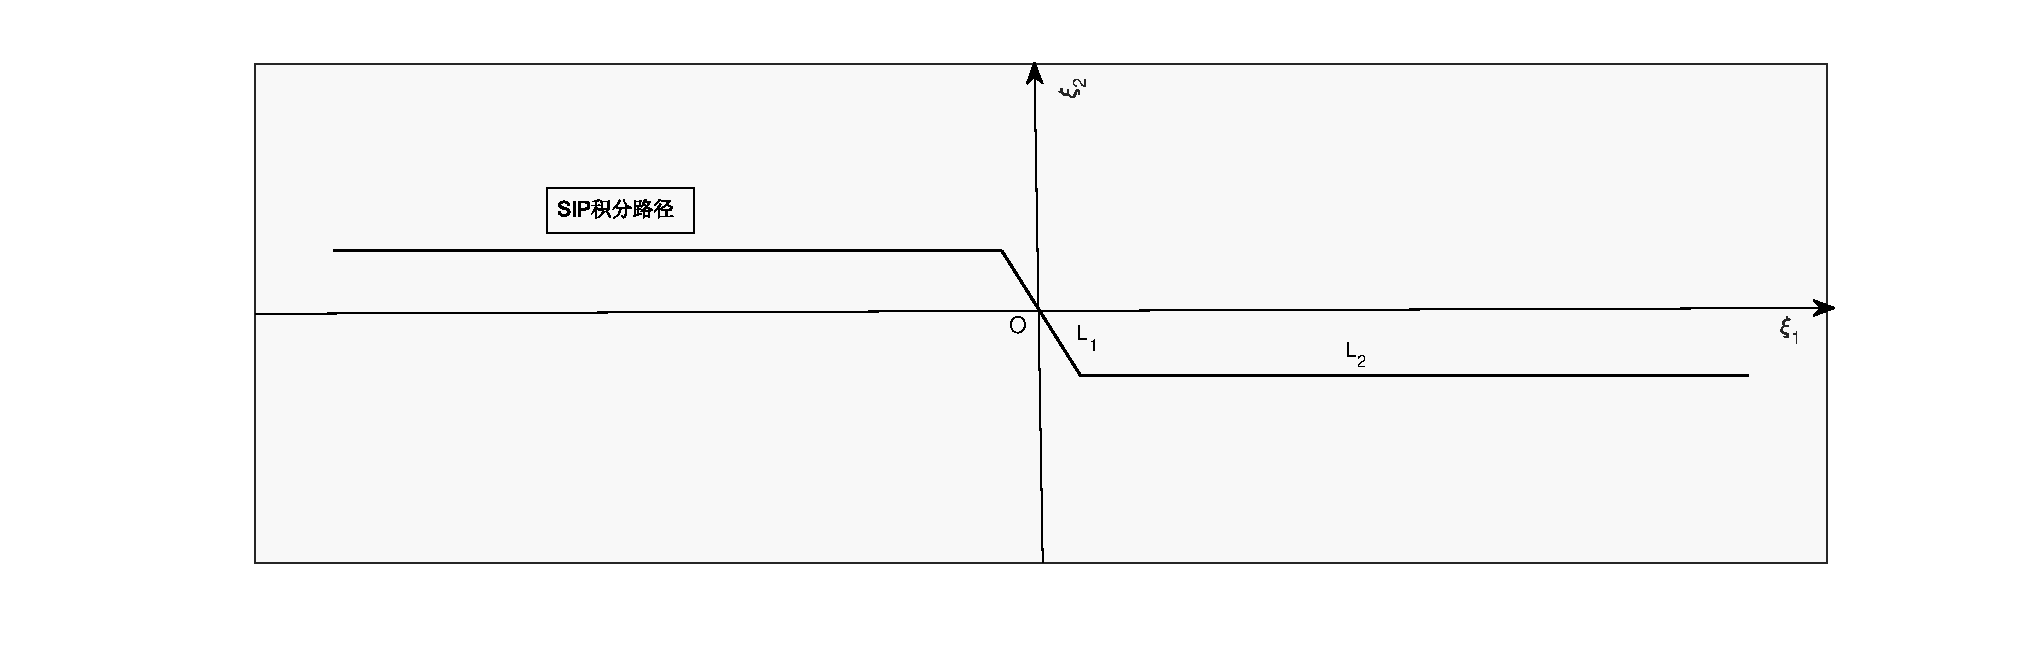
\includegraphics[width=15cm,height=6cm]{./SIP/SIP_path.eps}
  \caption{SIP积分路径}\label{SIP_path3}
\end{figure}


上一章提出的开波导逆时偏移算法的困难之处在于开波导模型本身就会产生波导模式,这从Neumann格林函数即可看出,而作为反传播的Dirichlet格林函数同样会产生波导模式,两者相互作用会使问题变得极为复杂。当$\lambda>0$时,Impedance格林函数$G_{\lambda}(x,y)$ 不会存在波导模式,从而为解决这一问题提供了可能。

除此之外,因为Impedance格林函数的表达式非常复杂,很难进行分析,因此在本节最后,我们将列出以$\Gamma_h$为间断面的全空间两层Hemholtz方程基本解$G_h(x,y)$ 的表达式。我们将看到函数$G_h(x,y)$不会产生波导模式,且波数与Pekeris开波导模型相符合,如果仅考虑Pekeris半空间两层开波导障碍物成像问题,或许可以考虑采用$G_h(x,y)$作为一种备选的反传播函数。全空间两层基本解 $G_h(x,y)$ 满足如下方程:
\begin{eqnarray}
\left\{
\begin{array}{lll}
  \Delta_xG_h(x,y)+\hat k^2(x)G_h(x,y)=-\delta_y(x),& in& \R^2\\
  & &\\
  \left[G_h(\cdot,y)\right]_{\Gamma_h}=\left[\frac{\partial G_h(\cdot,y)}{\partial\nu}\right]_{\Gamma_h}=0.
    \end{array}
\right.
\end{eqnarray}
其中波数$\hat k(x)$满足
\begin{eqnarray*}
\hat k(x)=\left\{
\begin{array}{lll}
  k_1&,&x_2<h\\
  k_2&,&x_2>h
\end{array}
\right.
\end{eqnarray*}
类似于文献\cite{cz2010,Desanto1992Scalar,Ammari2005A},直接计算可得$G_h(x,y)$ 的表达式如下:
\begin{lemma}\label{f_twolayer}
设积分路径$SIP$曲线如图\ref{SIP_path3} 所示,则函数$G_h(x,y)$表达式如下
\begin{eqnarray}
G_h(x,y)=\left\{
 \begin{array}{lll}
 \Phi(k_1,x,y)-\Phi(k_1,x,y^*)+P_{11}(x,y),& &y_2<h,x_2<h\\
 P_{12}(x,y),& &y_2<h,x_2>h\\
 P_{21}(x,y),& &y_2>h,x_2<h\\
 \Phi(k_2,x,y)-\Phi(k_2,x,y^*)+P_{22}(x,y),& &y_2>h,y_2>h
 \end{array}
 \right.
\end{eqnarray}
其中$y^*=(y_1,2h-y_2)$,$\mu_j=\sqrt{k_j^2-\xi^2}, j=1,2$,以及函数$P_{ij}(x,y)$的表达式为
\begin{eqnarray}
 \left\{
 \begin{array}{lll}
 P_{11}(x,y)&=&\frac{\i}{2\pi}\int_{SIP}\frac{1}{\mu_1+\mu_2}e^{\i\mu_1(2h-x_2-y_2)+\i\xi(x_1-y_1)}d\xi\\
 & &\\
 P_{12}(x,y)&=&\frac{\i}{2\pi}\int_{SIP}\frac{1}{\mu_1+\mu_2}e^{\i\mu_1(h-y_2)+\i\mu_2(x_2-h)+\i\xi(x_1-y_1)}d\xi\\
 & &\\
 P_{21}(x,y)&=&\frac{\i}{2\pi}\int_{SIP}\frac{1}{\mu_1+\mu_2}e^{\i\mu_2(y_2-h)+\i\mu_1(h-x_2)+\i\xi(x_1-y_1)}d\xi\\
 & &\\
 P_{22}(z,y)&=&\frac{\i}{2\pi}\int_{SIP}\frac{1}{\mu_1+\mu_2}e^{\i\mu_2(x_2+y_2-2h)+\i\xi(x_1-y_1)}d\xi
 \end{array}
 \right.
\end{eqnarray}
\end{lemma}

\section{点扩散函数}
在上一章中,我们参考文献\cite{ch_ha,ch_cw}中的逆时偏移算法,提出了Pekeris开波导逆时偏移算法\ref{alg_wg},该算法选取Pekeris开波导Dirichlet零边界Green函数进行反传播和计算互相关,能够很好地求解Pekeris开波导障碍物成像问题。但是由于反传播函数和开波导模型本身都会产生波导模式而导致当孔穴半径趋于无穷时,成像函数绝对收敛性无从保证。当$\lambda>0$时,Impedance格林函数$G_{\lambda}(x,y)$ 不存在波导模式,下面我们通过对点扩散函数进行分析和测试,来考量$G_{\lambda}(x,y)$是否可以解决我们的问题。

设源点$y\in\R^2_+$,以及$N(x,y)$为方程\eqref{G_Neumann}所定义的Pekeris开波导Neumann零边界的格林函数。然后令$x_r,r=1,2,\ldots,N_r$为均匀分布在$\Gamma_0^d$上的$N_r$个接收点,其中$d>0$为孔穴半径,以及$\Gamma_0^d:=\{(x_1,x_2)\in\R^2;x_1\in(-d,d),x_2=0\}$。则此时$\hat J_d(z,y)$为
\begin{equation}
 \hat J_d(z,y):=\frac{|\Gamma_0^d|}{N_r}\sum\limits_{r=1}^{N_r}\frac{\partial G_{\lambda}(x_r,z)}{\partial x_2(x_r)}\overline{N(x_r,y)}
\end{equation}
相应地接收点的个数$N_r\rightarrow\infty$时,我们得到有限孔穴点扩散函数$J_d(z,y)$,
\begin{equation}
  J_d(z,y):=\int_{\Gamma_0^d}\frac{\partial G_{\lambda}(x_r,z)}{\partial x_2(x_r)}\overline{N(x_r,y)}ds(x_r)
\end{equation}

假设$\lambda=2k_1,k_1=4\pi,k_2=2\pi,h=10,d=50,N_r=201$,源点$y_1=(0,8)$和$y_2=(0,12)$分别位于开波导第一层和第二层,
以及采样区域$\Omega=[-2,2]\times[6,14]$。测试结果如图\ref{fig_psf_impedance}所示,结果表明:无论是位于开波导第一层$L_1$内的源点,还是位于开波导第二层$L_2$内的源点,当选取的反传播函数为$G_{\lambda}$时,有限孔穴点扩散函数$J_d(z,y)$都能够很好地将点源$y$的位置给确定下来。

除此之外,我们也同时考虑了反传播函数为全空间两层基本解$G_h(x,z)$时,如下函数:
\begin{equation}
  \hat J_d^h(z,y):=\frac{|\Gamma_0^d|}{N_r}\sum\limits_{r=1}^{N_r}\frac{\partial G_h(x_r,z)}{\partial x_2(x_r)}\overline{N(x_r,y)}
\end{equation}
的测试情况,结果如图\ref{fig_psf_twolayer}所示。从数值测试结果来看,除了函数的具体值大小有所区别,取$G_h(x,z)$为反传播函数能够达到和之前取$G_{\lambda}(x,z)$时相同的效果。虽然该方法无法推广到半空间开波导任意层,不过如果仅考虑半空间两层开波导模型下的障碍物成像问题,或许可以将其作为一个备选方案,其优点是函数表达式相对简单,理论分析和数值测试相对容易进行。
\begin{figure}[h]
  \centering
  \includegraphics[width=13cm,height=5cm]{./waveguide1/psf_waveguide/in_mesh.eps}
    \includegraphics[width=13cm,height=5cm]{./waveguide1/psf_waveguide/out_mesh.eps}
  \caption{反传播函数为$G_{bp}(x,z)=G_{\lambda}(x,z)$时的有限孔穴点扩散函数的负虚部:$-\Im J_d(z,y)$,其中第一行为源点$y_1=(0,8)$在$ L_1$中,第二行为源点$y_2=(0,12)$在$ L_2$中,采样区域$\Omega$为$[-2,2]\times[6,14]$.}\label{fig_psf_impedance}
\end{figure}
\begin{figure}[h]
  \centering
  \includegraphics[width=13cm,height=5cm]{./waveguide1/psf_twolayer/in_mesh.eps}
    \includegraphics[width=13cm,height=5cm]{./waveguide1/psf_twolayer/out_mesh.eps}
  \caption{反传播函数为$G_{bp}(x,z)=G_h(x,z)$时的有限孔穴点扩散函数的负虚部:$-\Im J_d(z,y)$,其中第一行为源点$y_1=(0,8)$在$ L_1$中,第二行为源点$y_2=(0,12)$在$ L_2$中,采样区域$\Omega$为$[-2,2]\times[6,14]$.}\label{fig_psf_twolayer}
\end{figure}

\section{阻抗型开波导逆时偏移算法}
根据对点扩散函数的测试,我们提出适用于开波导模型的阻抗型逆时偏移算法:
\begin{algorithm}\label{alg_imp}
设$\Omega$为采样区域,令$u^s(x_r,x_s)$ 为在接收点$x_r$收到的由源点$x_s$所激发的散射数据,其中$x_r,x_s\in\Gamma_0^d;r=1,\ldots,N_r;s=1,\ldots,N_s$.\\
$1^\circ$ 反传播: 对$s=1,\ldots,N_s$,计算反传播场
\begin{equation}
  v_b(z,x_s)=\frac{|\Gamma_0^d|}{N_r}\sum\limits_{r=1}^{N_r}\frac{\partial G_{\lambda}(x_r,z)}{\partial x_2(x_r)}\overline{u^s(x_r,x_s)},\  \  \forall z\in\Omega.
\end{equation}
若令$N_r\rightarrow0$,则上式可看做如下积分的数值近似,
\begin{equation}
  \hat v_b(z,x_s)=\int_{\Gamma_0^d}\frac{\partial G_{\lambda}(x_r,z)}{\partial x_2(x_r)}\overline{u^s(x_r,x_s)}ds(x_r)
\end{equation}
$2^\circ$ 互相关: 对$z\in\Omega$,计算成像函数
\begin{equation*}
  I_d(z)=\Im\left\{\frac{|\Gamma_0^d|}{N_s}\sum\limits_{s=1}^{N_s}\frac{\partial G_{\lambda}(x_s,z)}{\partial x_2(x_s)}v_b(z,x_s)
  \right\}.
\end{equation*}
将$v_b(z,x_s)$的表达式代入,可得
\begin{equation}\label{Id_imp}
  I_d(z)=\Im\left\{\frac{|\Gamma_0^d|}{N_s}\frac{|\Gamma_0^d|}{N_r}\sum\limits_{s=1}^{N_s}\sum\limits_{r=1}^{N_r}\frac{\partial G_{\lambda}(x_s,z)}{\partial x_2(x_s)}\frac{\partial G_{\lambda}(x_r,z)}{\partial x_2(x_r)}\overline{u^s(x_r,x_s)}
  \right\}.
\end{equation}
成像函数\eqref{Id_imp}将用于下节所有的数值算例测试。
若令$N_s,N_r\rightarrow\infty$,则上式可看做如下积分的数值近似,
\begin{equation}\label{Idhat_imp}
  \hat I_d(z)=\Im\int_{\Gamma_0^d}\int_{\Gamma_0^d}\frac{\partial G_{\lambda}(x_s,z)}{\partial x_2(x_s)}
  \frac{\partial G_{\lambda}(x_r,z)}{\partial x_2(x_r)}\overline{u^s(x_r,x_s)}ds(x_r)ds(x_s).
\end{equation}
\end{algorithm}

\begin{remark}
算法\ref{alg_imp}相比于算法\ref{alg_wg}的优点在于,我们多了一个参数$\lambda$,从而具有了更好的灵活性。通过对边界阻抗常数$\lambda$的合理选取,如$\lambda>0$,可使得反传播函数$G_{\lambda}$不存在波导模式,从而避免了问题\ref{pro_convergence}。除此之外,如果仅考虑Pekeris半空间两层开波导障碍物成像问题,算法\ref{alg_imp}中的反传播函数$G_{\lambda}(x,z)$可以考虑替换成全空间两层基本解$G_h(x,z)$,其中函数$G_h(x,z)$的具体表达式见引理\ref{f_twolayer}。
\end{remark}
\section{数值测试}
下面我们对算法\ref{alg_imp}进行数值测试,本章依旧采用具有参数表示的障碍物边界作为测试算例,分别为$P$叶风扇形状、 圆形、花生形状以及边角被光滑后的方块形状,其参数表达分别如下
\begin{eqnarray}\label{obstacle_example2}
\left\{
\begin{array}{lll}
x_1=r(\theta)\cos\theta&,& x_2=r(\theta)\sin\theta,\ \ \mbox{其中}\ \ r(\theta)=1+0.2\cos(p\theta),\\
x_1=\rho\cos{\theta}&,& x_2=\rho\sin{\theta},\\
x_1=\cos{\theta}+0.2\cos{3\theta}&,& x_2=\sin{\theta}+0.2\sin{3\theta},\\
x_1=\cos^3\theta+\cos{\theta}&,& x_2=\sin^3\theta+\sin{\theta}.
\end{array}
\right.
\end{eqnarray}
\subsection{$D\subset L_1$.}

在本小节,我们测试当障碍物位于开波导第一层时,算法\ref{alg_imp}的成像效果。假设$h=10$以及$d=50$,并且源点和接收点均匀分布在$\Gamma_0^d$ 上,
$$
 x_{1s}=-d+\frac{2d}{N_s}(s-1)+\frac{d}{N_s},\  \ x_{1r}=-d+\frac{2d}{N_r}(r-1),\ \
$$
其中$s=1,\ldots,N_s, r=1,\ldots,N_r$,以及$\Gamma_0^d=\{(x_1,x_2)\in\R^2;x_1\in(-d,d),x_2=0\}$。此外,假设采样区域为$\Omega=[-2,2]\times[6,10]$,且我们采用$201\times201$的均匀采样。阻抗系数$\lambda=2 k_1$,探测频率单频时为$k_1=4\pi,k_2=2\pi$。 源点和接收点个数为$N_s=256,N_r=256$。

\begin{example}[不同形状]\label{imp_ex1}
在本算例中,我们以声软障碍物和可穿透障碍物为例测试了位于开波导不同位置的具有不同形状的障碍物,例如4叶风扇形状,矩形形状,花生形状和椭圆形状,算法\ref{alg_imp}的成像效果。与此同时,我们也测试了当所采用的反传播函数为全空间两层基本解$G_h(x,z)$,如下成像函数:
\begin{equation}\label{Id_twolayer}
   I_d^h(z)=\Im\left\{\frac{|\Gamma_0^d|}{N_s}\frac{|\Gamma_0^d|}{N_r}\sum\limits_{s=1}^{N_s}\sum\limits_{r=1}^{N_r}\frac{\partial G_h(x_s,z)}{\partial x_2(x_s)}\frac{\partial G_h(x_r,z)}{\partial x_2(x_r)}\overline{u^s(x_r,x_s)}
  \right\}.
\end{equation}
的成像效果。

声软障碍物和可穿透障碍物的测试结果分别如图\ref{fig_imp_ex1_1}和\ref{fig_imp_ex1_2}所示,其中第一行为算法\ref{alg_imp}中函数\ref{Id_imp}的成像效果,第二行为取反传播函数为全空间两层基本解$G_h(x,z)$时的成像函数\ref{Id_twolayer}的成像效果。结果表明:当障碍物$D$位于开波导第一层$L_1$时,除了成像值有所区别之外,两种成像函数都能够对不同形状的障碍物进行有效成像,而且成像效果与算法\ref{alg_wg}几乎都达到了相同的效果。除此之外,我们也看到了,对于可穿透障碍物的成像效果要稍微好于声软障碍物。
\end{example}

\begin{figure}[h]
  \centering
  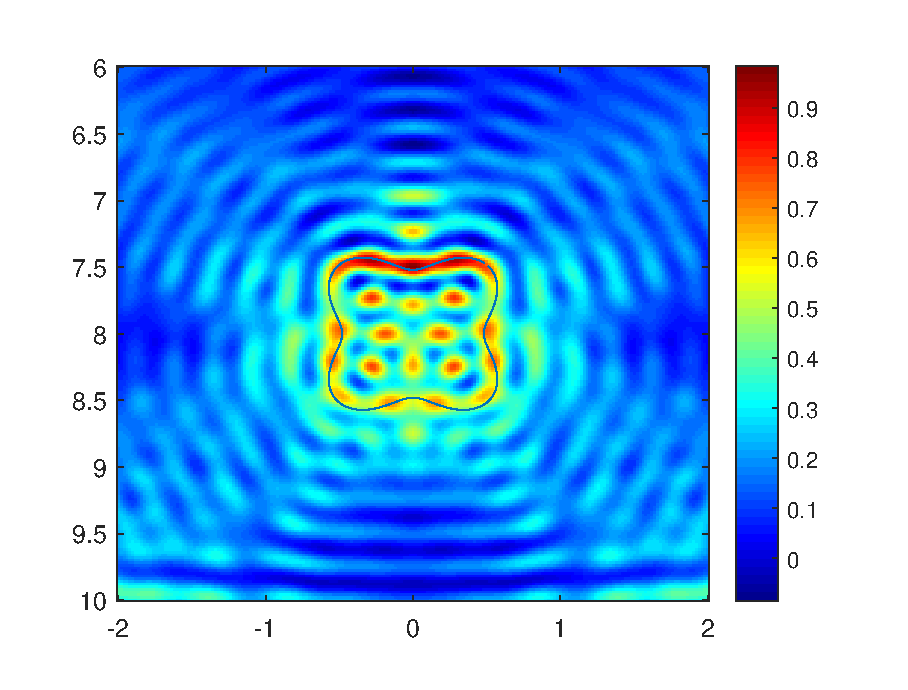
\includegraphics[width=0.23\textwidth]{./waveguide2/example1/pleaf1_soft_in_impedance.eps}
  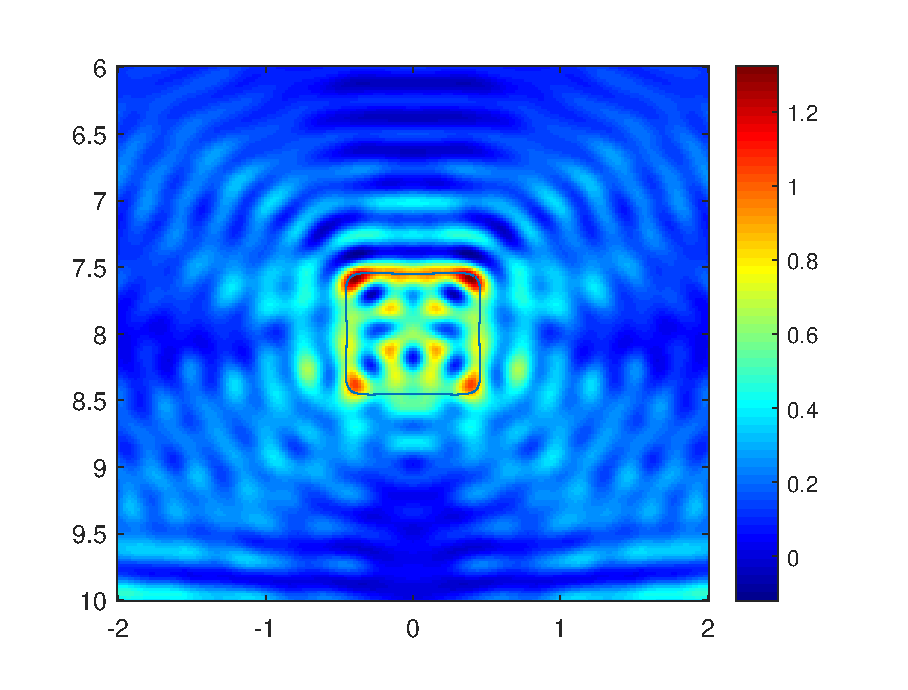
\includegraphics[width=0.23\textwidth]{./waveguide2/example1/square1_soft_in_impedance.eps}
  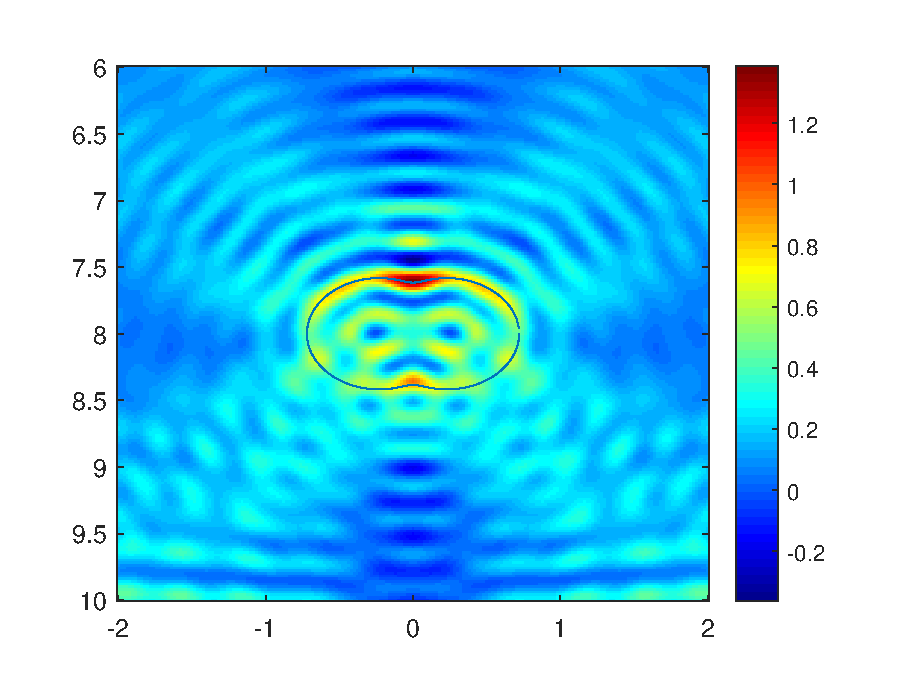
\includegraphics[width=0.23\textwidth]{./waveguide2/example1/peanut_soft_in_impedance.eps}{\tiny }
  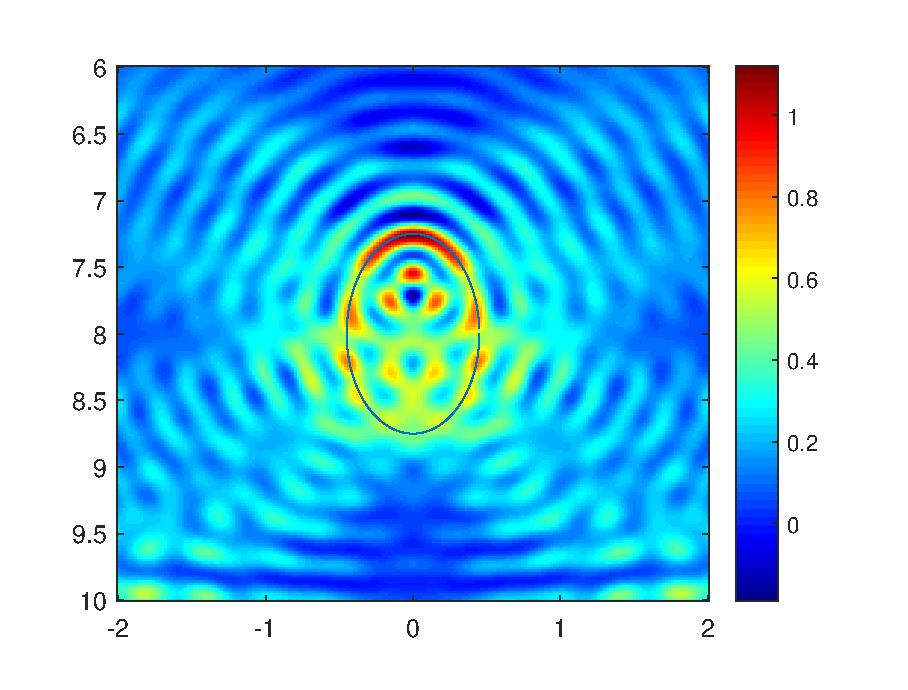
\includegraphics[width=0.23\textwidth]{./waveguide2/example1/circle1_soft_in_impedance.eps}\\
  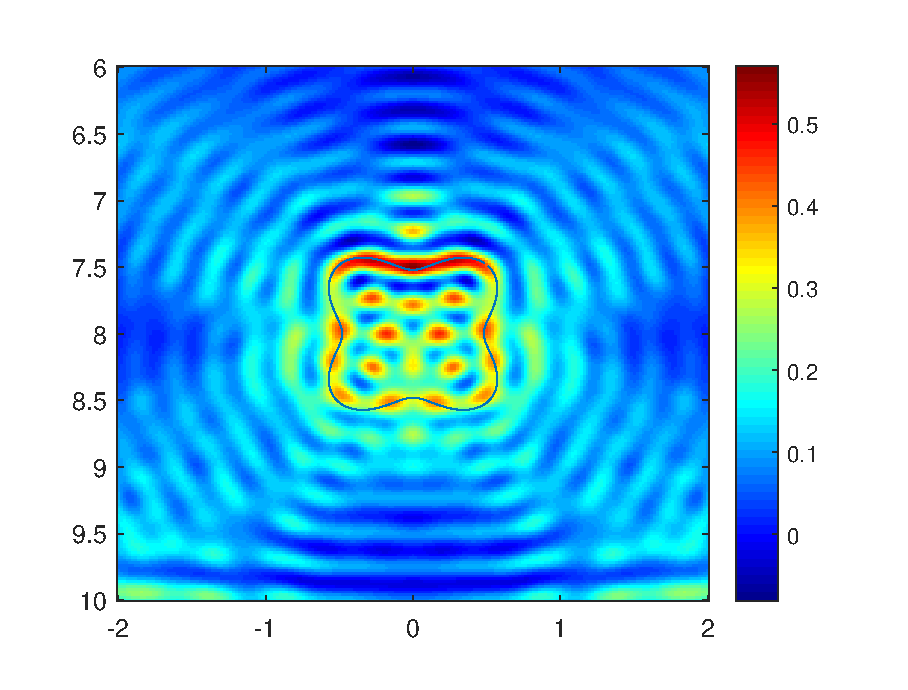
\includegraphics[width=0.23\textwidth]{./waveguide2/example1/pleaf1_soft_in_twolayer.eps}
  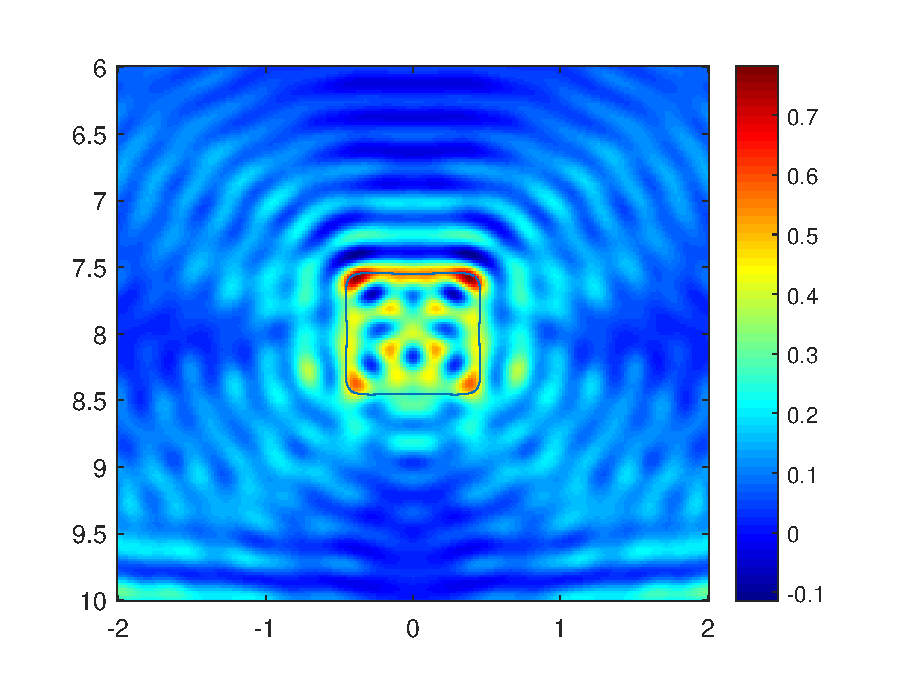
\includegraphics[width=0.23\textwidth]{./waveguide2/example1/square1_soft_in_twolayer.eps}
  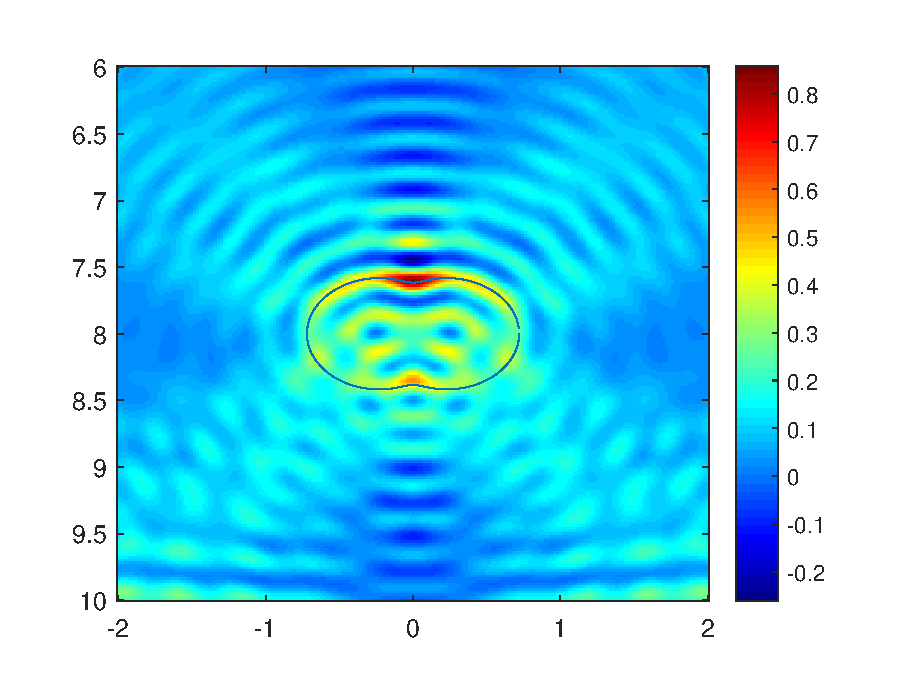
\includegraphics[width=0.23\textwidth]{./waveguide2/example1/peanut_soft_in_twolayer.eps}
  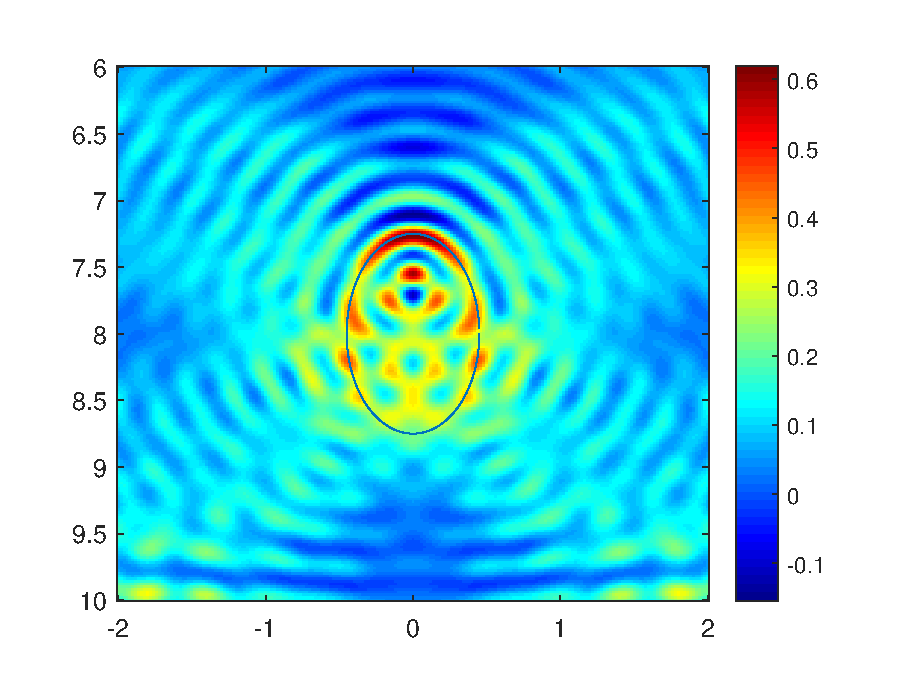
\includegraphics[width=0.23\textwidth]{./waveguide2/example1/circle1_soft_in_twolayer.eps}
  \caption{算例\ref{imp_ex1}:测试不同形状的声软障碍物:从左到右依次为4-叶风扇、矩形、花生以及椭圆形状,其中第一行是算法\ref{alg_imp}中函数\ref{Id_imp}的成像效果,第二行为取反传播函数为$G_h(x,z)$的函数\ref{Id_twolayer}的成像效果。}\label{fig_imp_ex1_1}
\end{figure}
\begin{figure}[h]
	\centering
	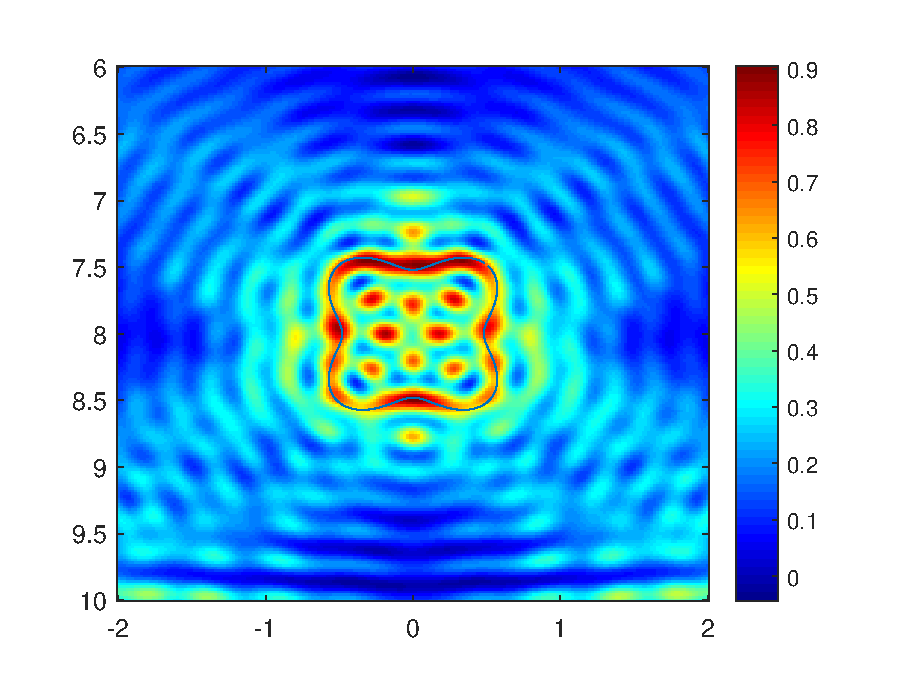
\includegraphics[width=0.23\textwidth]{./waveguide2/example1/pleaf1_tran_in_impedance.eps}
	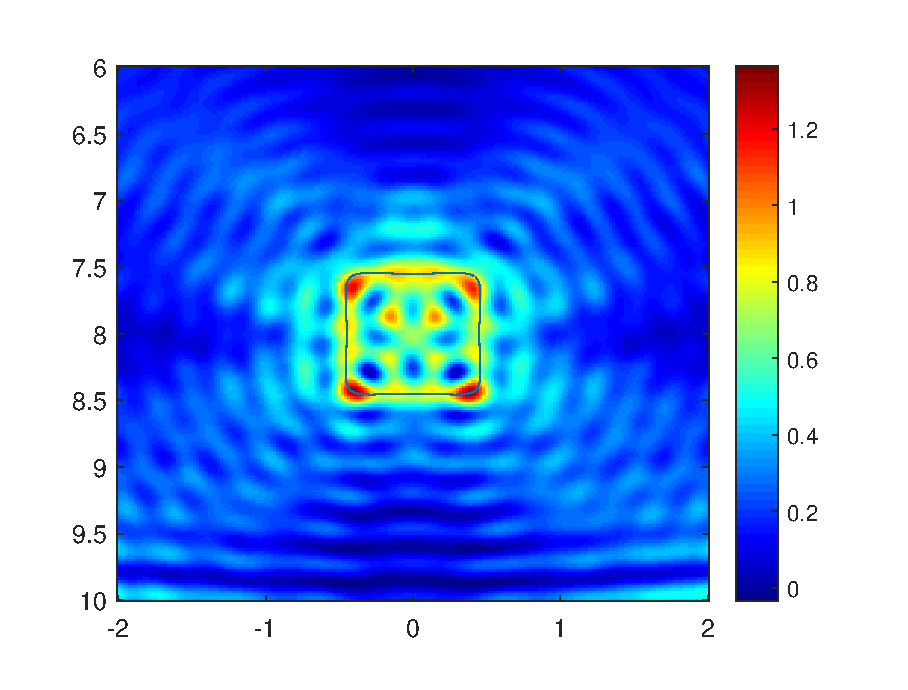
\includegraphics[width=0.23\textwidth]{./waveguide2/example1/square1_tran_in_impedance.eps}
	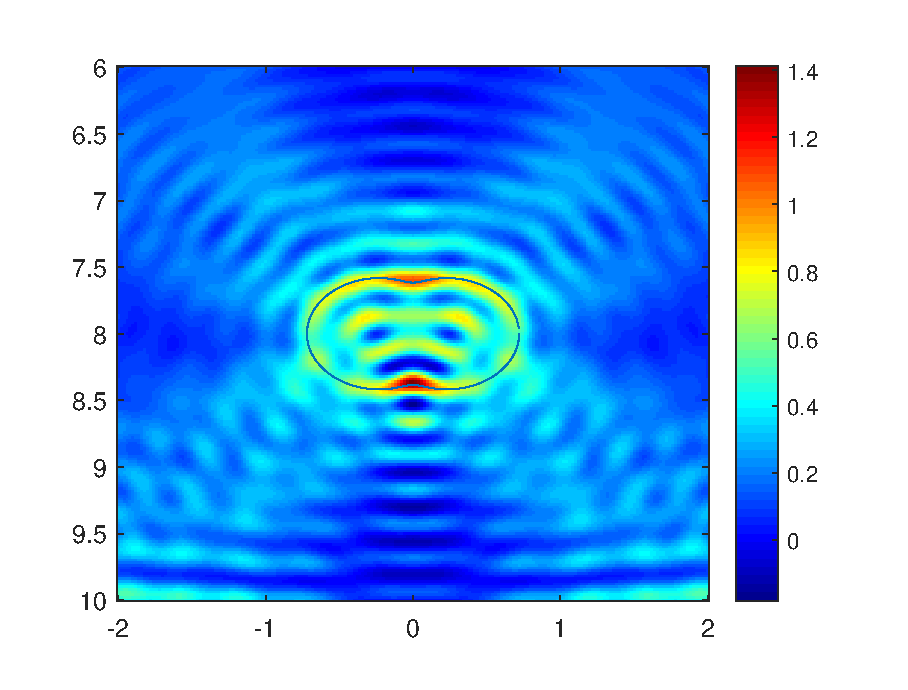
\includegraphics[width=0.23\textwidth]{./waveguide2/example1/peanut_tran_in_impedance.eps}
	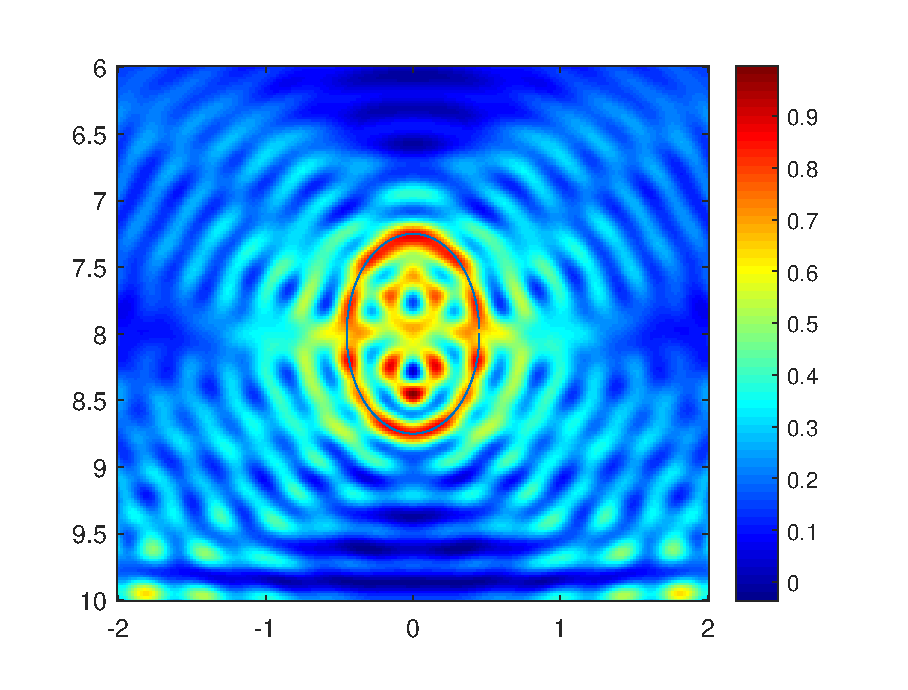
\includegraphics[width=0.23\textwidth]{./waveguide2/example1/circle1_tran_in_impedance.eps}\\
	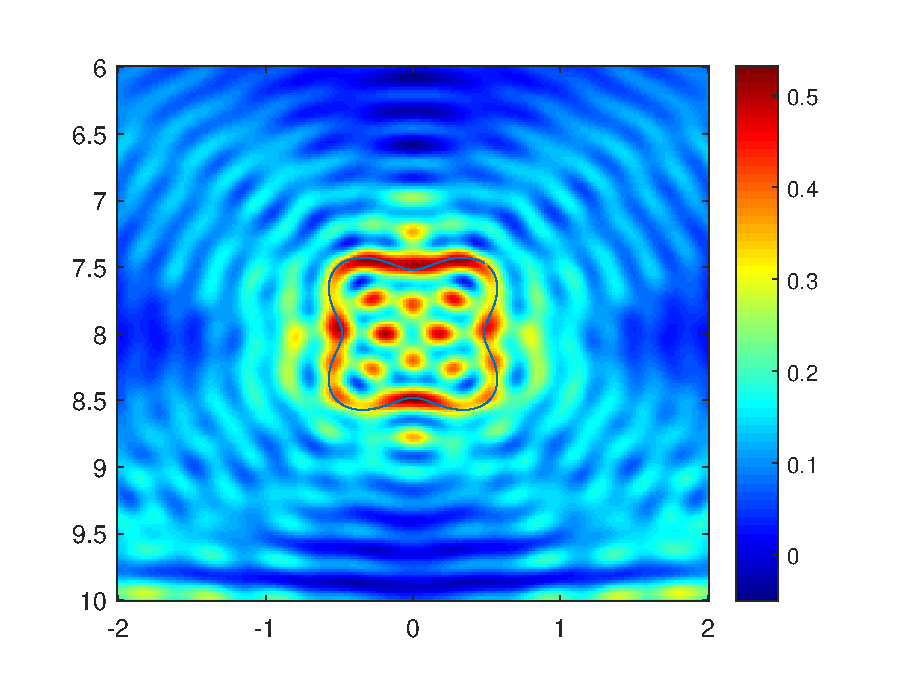
\includegraphics[width=0.23\textwidth]{./waveguide2/example1/pleaf1_tran_in_twolayer.eps}
	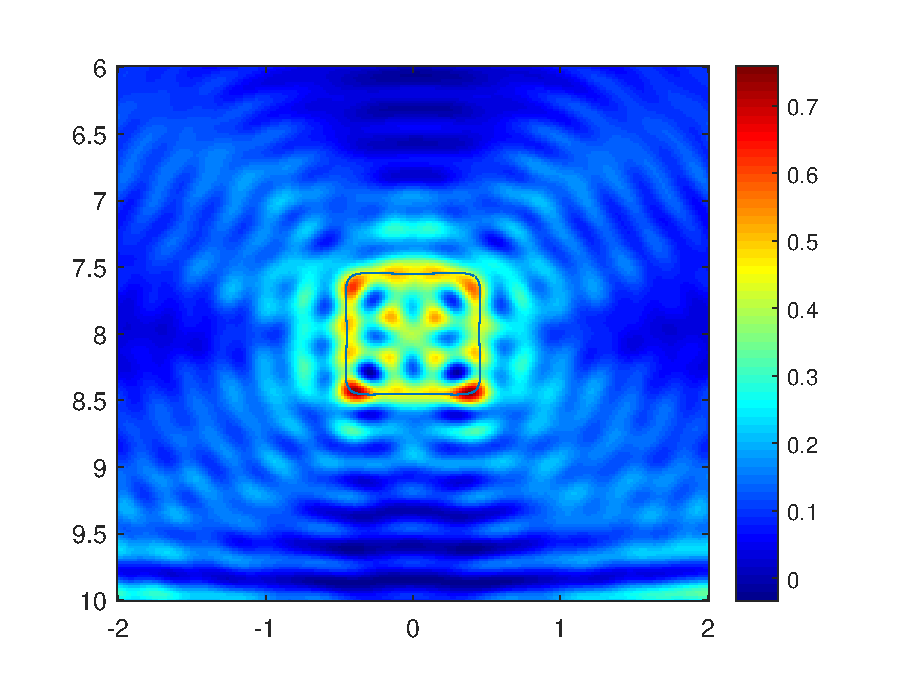
\includegraphics[width=0.23\textwidth]{./waveguide2/example1/square1_tran_in_twolayer.eps}
	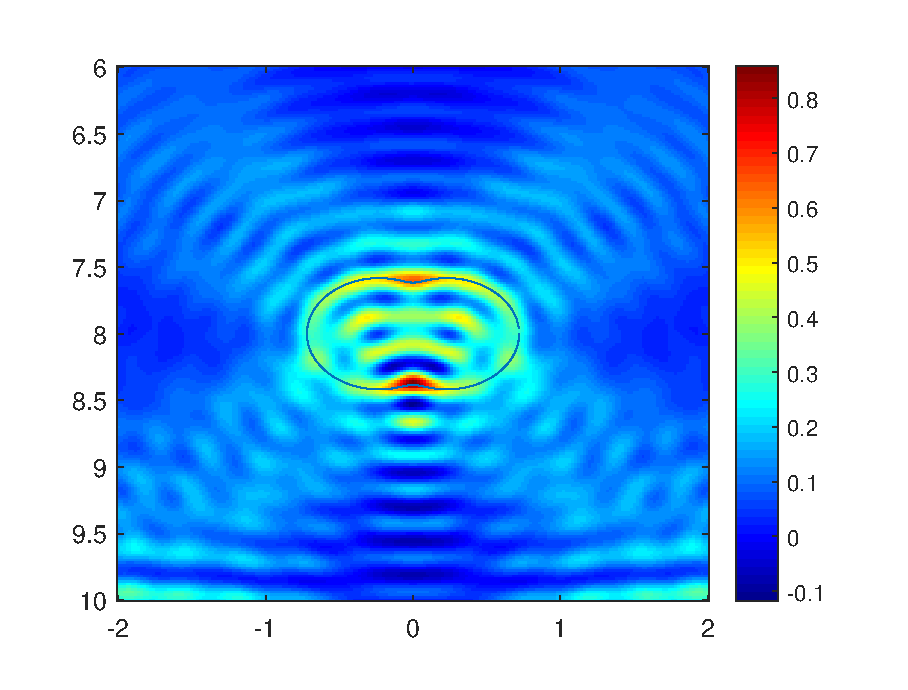
\includegraphics[width=0.23\textwidth]{./waveguide2/example1/peanut_tran_in_twolayer.eps}
	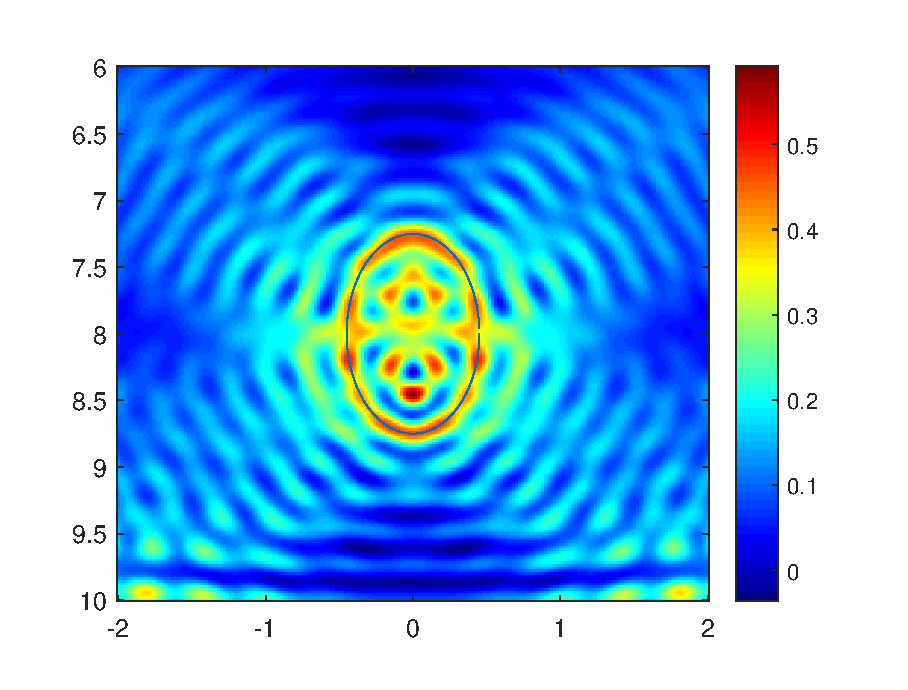
\includegraphics[width=0.23\textwidth]{./waveguide2/example1/circle1_tran_in_twolayer.eps}
	\caption{算例\ref{imp_ex1}:测试不同形状的可穿透障碍物:从左到右依次为4-叶风扇、矩形、花生以及椭圆形状,其中第一行是算法\ref{alg_imp}中函数\ref{Id_imp}的成像效果,第二行为取反传播函数为$G_h(x,z)$的函数\ref{Id_twolayer}的成像效果。}\label{fig_imp_ex1_2}
\end{figure}
\begin{example}[不同边界类型]\label{imp_ex2}
在本算例中,我们以圆形障碍物为例,验证算法\ref{alg_imp}对嵌入在Pekeris开波导中具有不同边界类型的障碍物的成像效果。例如声软障碍物,声硬障碍物,折射系数为$n(x)$ 的可穿透障碍物,阻尼系数为$\eta(x)$的阻抗边界障碍物。对于可穿透障碍物成像,我们假设折射系数$n(x)$ 为:
\begin{eqnarray*}
n(x)=\left\{
\begin{array}{lll}
  0.5&,&x\in D\\
  1&,&x\in\R_+^2\backslash\overline D
\end{array}
\right.
\end{eqnarray*}
对于阻抗边界障碍物,我们假设在上半边界$\eta(x)=1$,在下半边界$\eta(x)=2$。

测试效果如图\ref{fig_imp_ex2}所示,其中第一行为算法\ref{alg_imp}中函数\ref{Id_imp}的成像效果,第二行为取反传播函数为全空间两层基本解$G_h(x,z)$时的成像函数\ref{Id_twolayer}的成像效果。结果表明:在没有提前知道障碍物的任何先验信息的情况下,例如是否可穿透以及不可穿透障碍物的边界条件,算法\ref{alg_imp}以及成像函数\ref{Id_twolayer}都能够对不同类型的圆形障碍物做到有效成像。而且除了具体数值有所区别外,其成像效果与算法\ref{alg_wg}并无多大区别。
\end{example}

\begin{figure}[htbp]
  \centering
  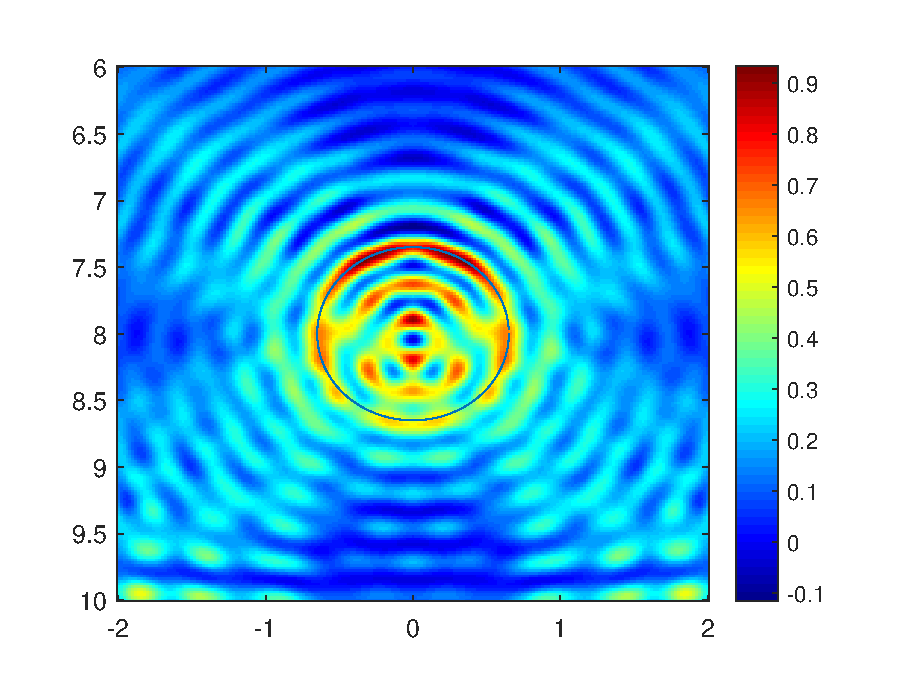
\includegraphics[width=0.23\textwidth]{./waveguide2/example2/circle_soft_in_impedance.eps}
  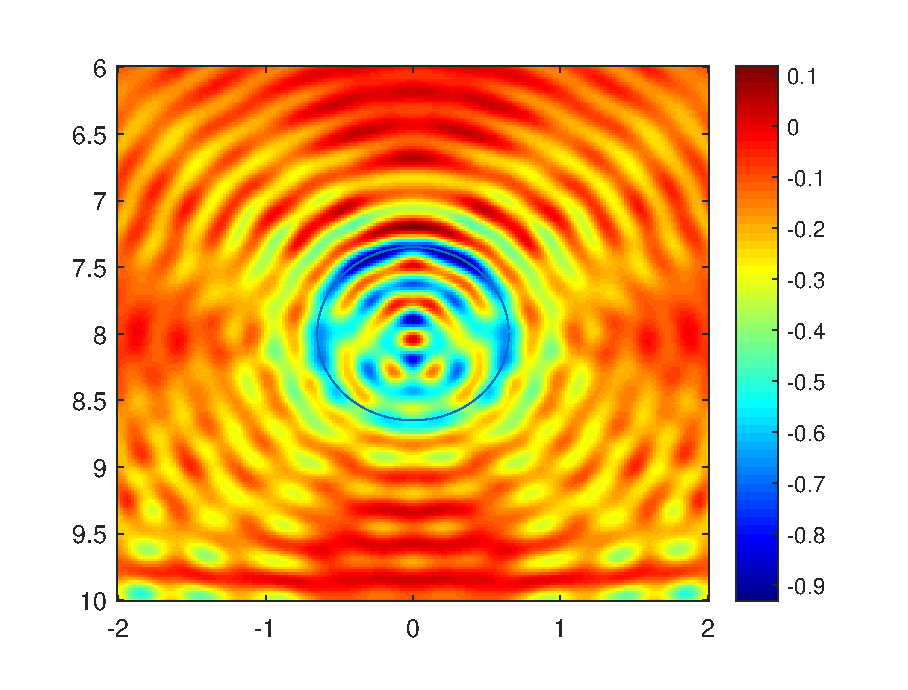
\includegraphics[width=0.23\textwidth]{./waveguide2/example2/circle_hard_in_impedance.eps}
  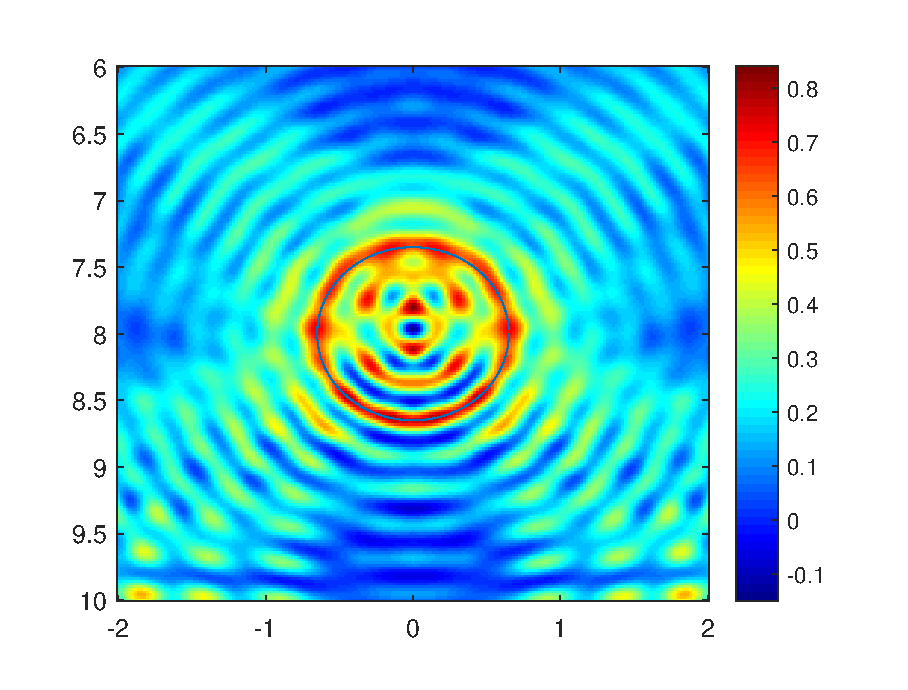
\includegraphics[width=0.23\textwidth]{./waveguide2/example2/circle_impedance_in_impedance.eps}
  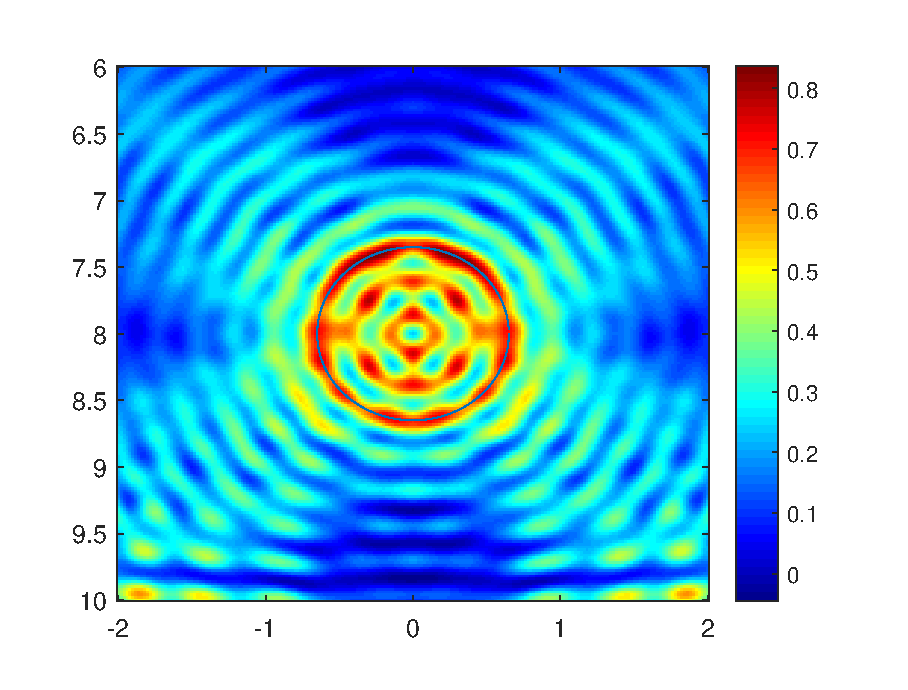
\includegraphics[width=0.23\textwidth]{./waveguide2/example2/circle_transmission_in_impedance.eps}
  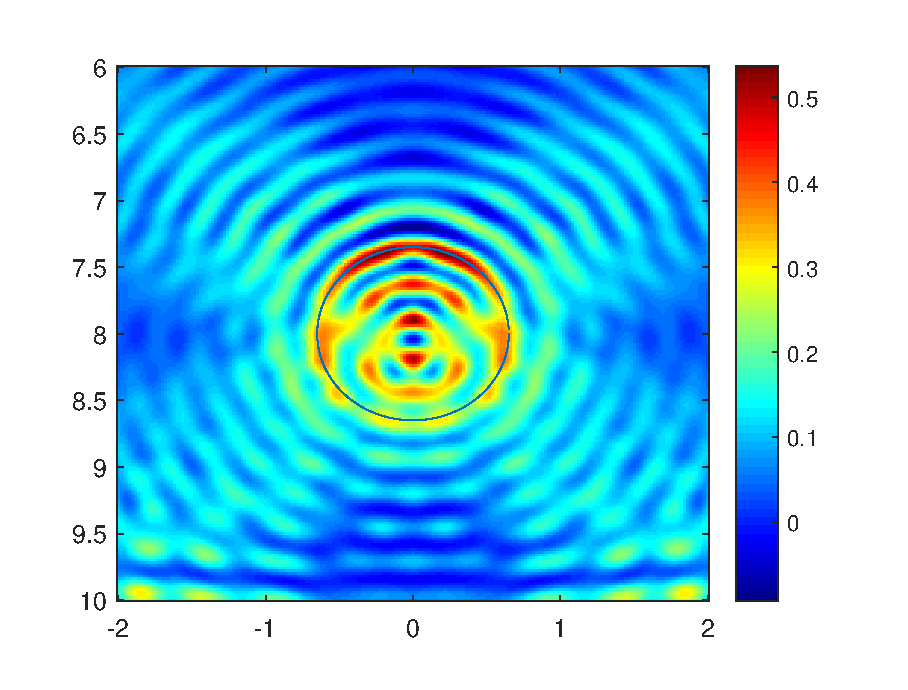
\includegraphics[width=0.23\textwidth]{./waveguide2/example2/circle_soft_in_twolayer.eps}
  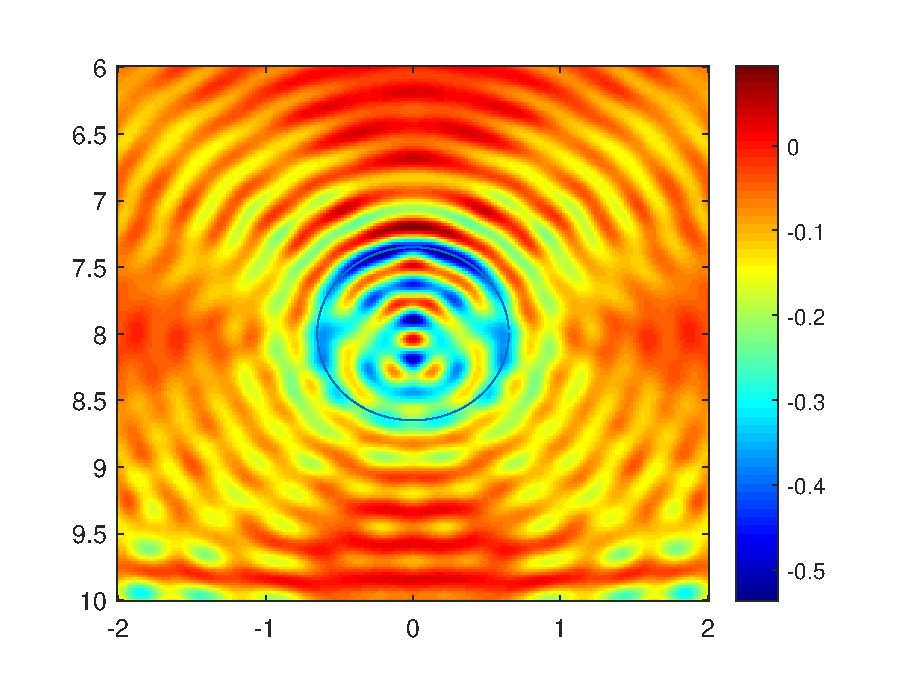
\includegraphics[width=0.23\textwidth]{./waveguide2/example2/circle_hard_in_twolayer.eps}
  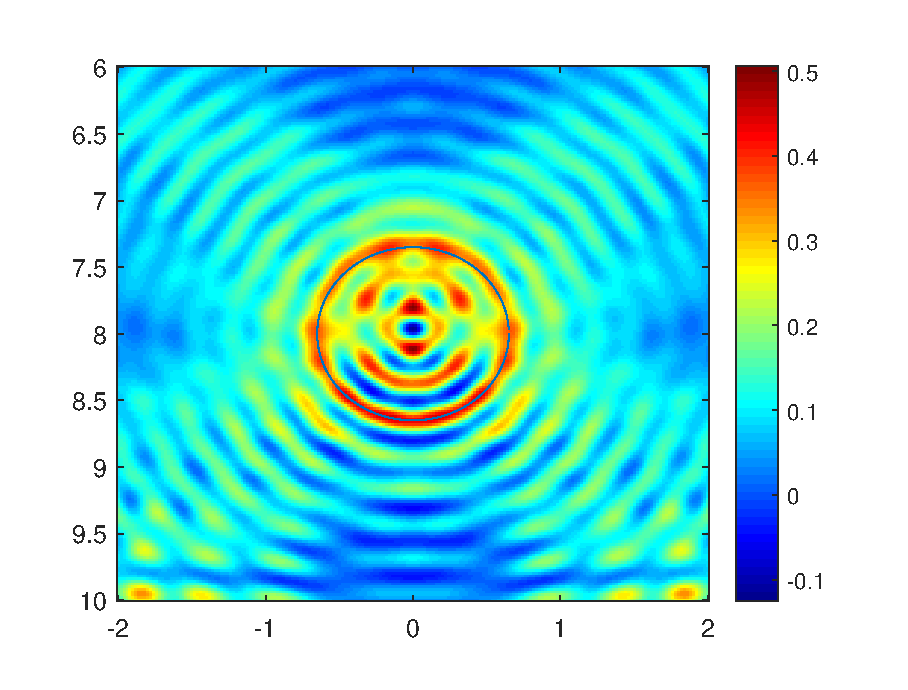
\includegraphics[width=0.23\textwidth]{./waveguide2/example2/circle_impedance_in_twolayer.eps}
  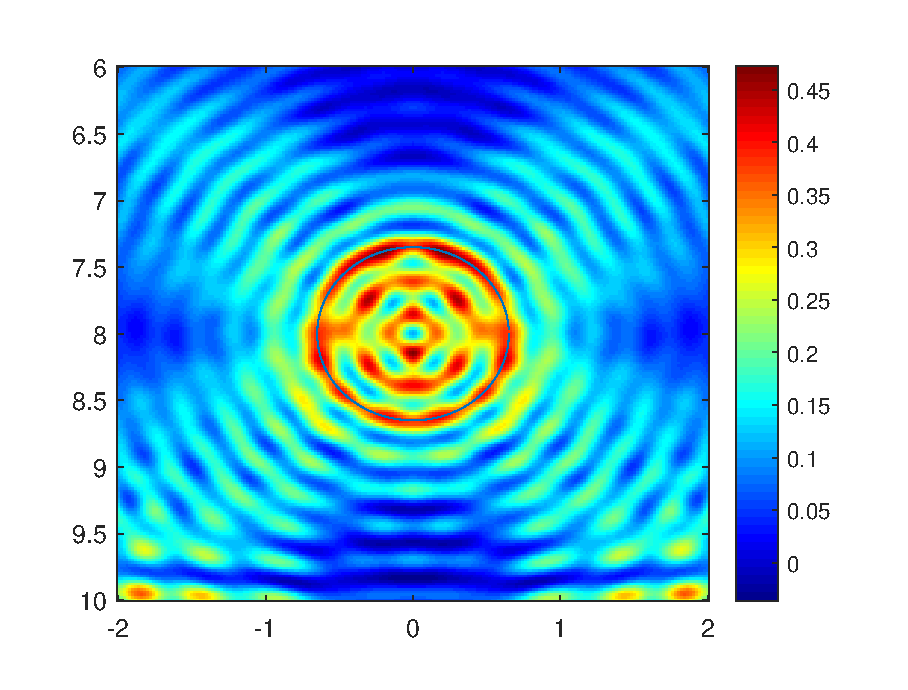
\includegraphics[width=0.23\textwidth]{./waveguide2/example2/circle_transmission_in_twolayer.eps}
  \caption{算例\ref{imp_ex2}:测试不同类型的圆形障碍物:从左到右依次为声软障碍物、声硬障碍物、阻尼系数为$\eta(x)$的阻抗边界障碍物以及折射系数为$n(x)$的可穿透障碍物,其中第一行是算法\ref{alg_imp}中函数\ref{Id_imp}的成像效果,第二行为取反传播函数为$G_h(x,z)$的函数\ref{Id_twolayer}的成像效果。}\label{fig_imp_ex2}
\end{figure}
\begin{example}[抗噪性单频测试]\label{imp_ex3}
在本算例中,我们测试当散射数据$u^s(x_r,x_s)$带有高斯噪音时,算法\ref{alg_imp}对位于Pekeris开波导第一层障碍物的成像效果。设$u^s_{noise}(x_r,x_s)$ 为如下带有高斯噪音的散射数据:
$$ u^s_{noise}(x_r,x_s)=u^s(x_r,x_s)+v_{noise},$$
其中$v_{noise}$为满足如下分布的高斯噪音:
$$v_{noise}=\mu \max{|u^s|}\epsilon,\ \ \epsilon\sim N(0,1).$$

假设噪音水平$\mu$按如下数值依次递增:$0.1,0.2,0.4,0.6$。分别采用单频和多频进行测试,其中单频参数设置为:$k_1=4\pi,k_2=2\pi,\lambda=2k_1$;多频时参数设置为:$\lambda=2k_1,k_2=\frac{1}{2}k_1,k_1=2\pi+0.4n\pi,n=0,1,\ldots,9$。

第一个测试为4-叶风扇形状的声软障碍物,第二个测试为圆形的可穿透障碍物,测试结果分别如图\ref{fig_imp_ex3_1}和图\ref{fig_imp_ex3_2}所示。结果表明:1. 算法\ref{alg_imp}中的成像函数\eqref{Id_imp}具有十分良好的抗噪音性能;2. 当在$\Gamma_0^d$所采集的数据为多频数据时,直接将多个频率的成像函数进行相加能够极大改善成像效果,提高抗噪音能力,这也同时间接表明了算法\ref{alg_imp}成像的准确性; 3. 对于可穿透障碍物的成像效果要稍微好于声软障碍物。
\end{example}

\begin{figure}[htbp]
  \centering
  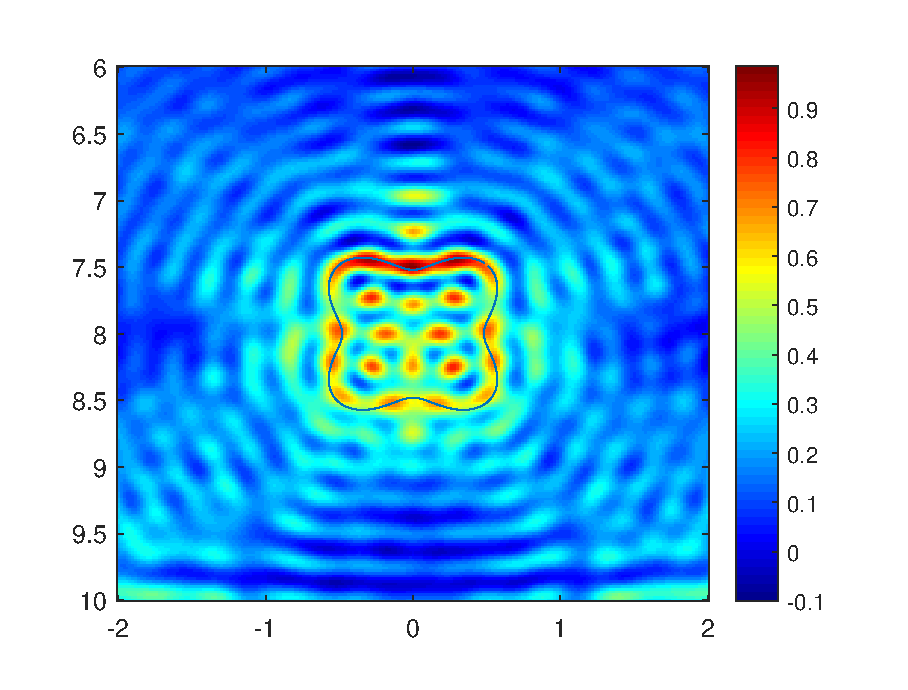
\includegraphics[width=0.23\textwidth]{./waveguide2/example3/pleaf1_soft_in_impedance2.eps}
  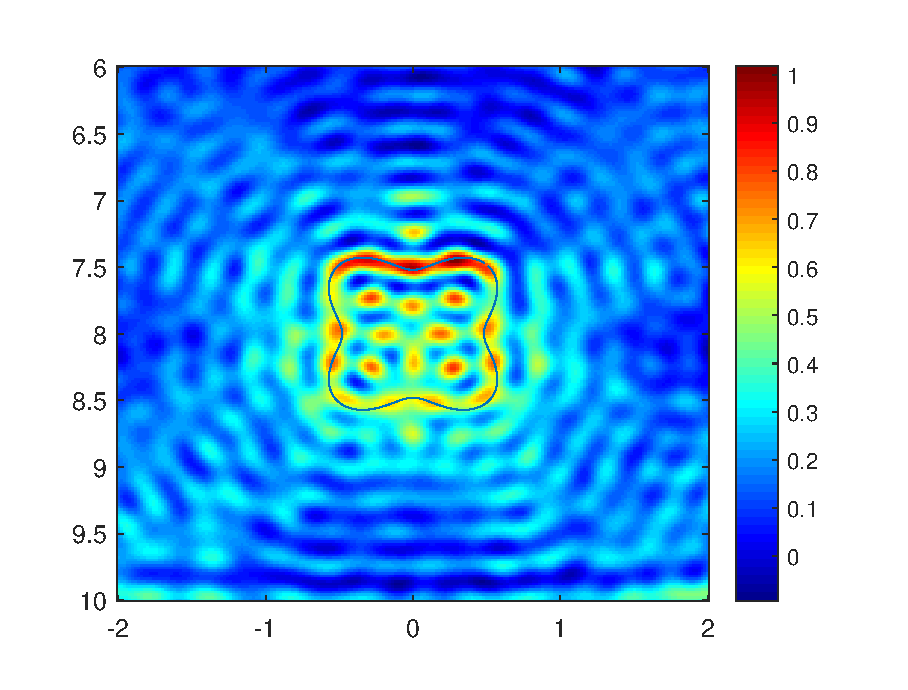
\includegraphics[width=0.23\textwidth]{./waveguide2/example3/pleaf1_soft_in_impedance4.eps}
  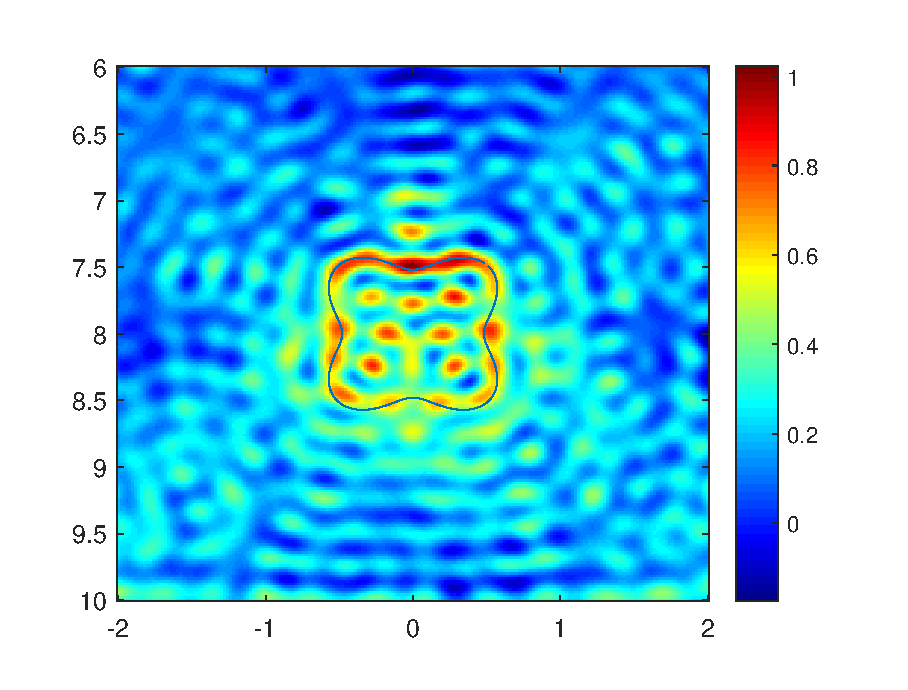
\includegraphics[width=0.23\textwidth]{./waveguide2/example3/pleaf1_soft_in_impedance6.eps}
  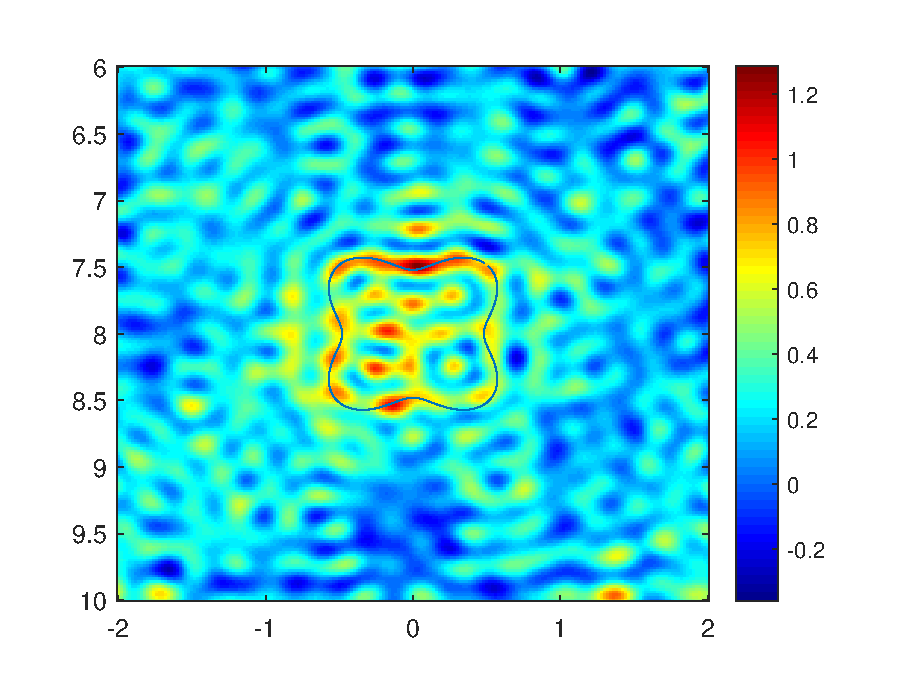
\includegraphics[width=0.23\textwidth]{./waveguide2/example3/pleaf1_soft_in_impedance8.eps}
  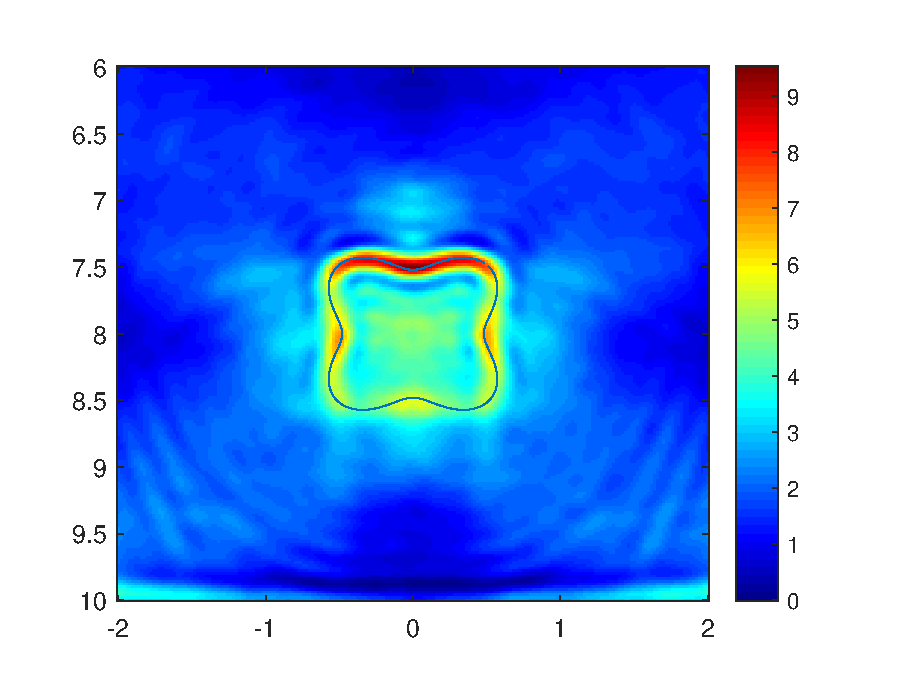
\includegraphics[width=0.23\textwidth]{./waveguide2/example3/pleaf1_soft_in_impedance2_mul.eps}
  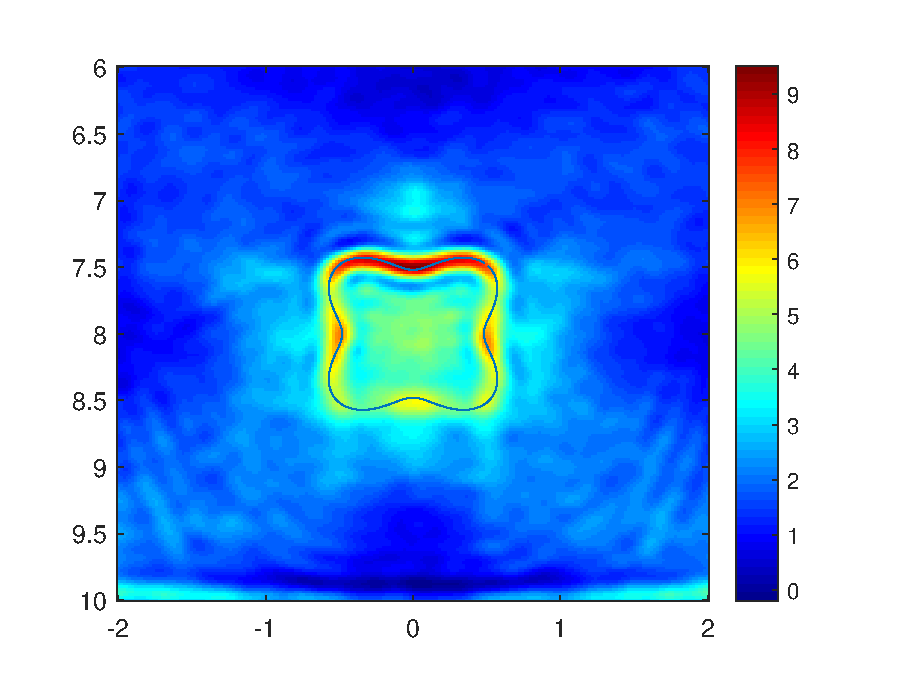
\includegraphics[width=0.23\textwidth]{./waveguide2/example3/pleaf1_soft_in_impedance4_mul.eps}
  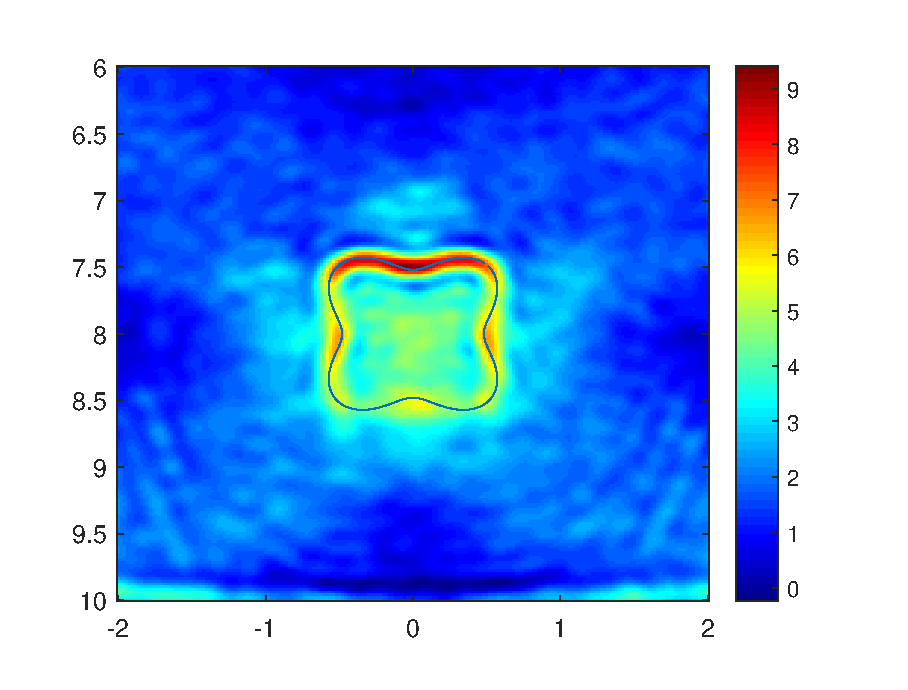
\includegraphics[width=0.23\textwidth]{./waveguide2/example3/pleaf1_soft_in_impedance6_mul.eps}
  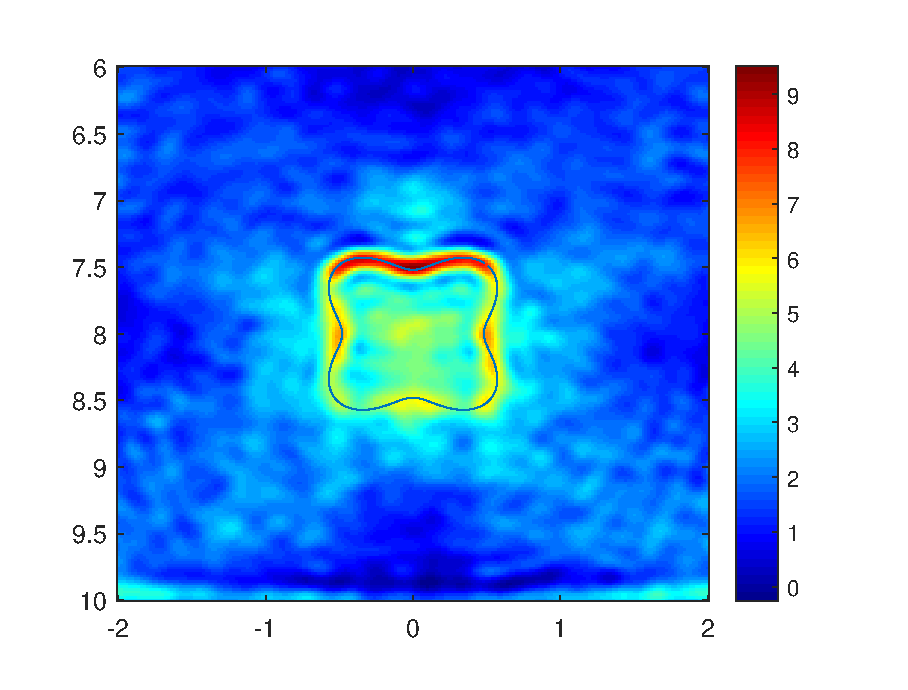
\includegraphics[width=0.23\textwidth]{./waveguide2/example3/pleaf1_soft_in_impedance8_mul.eps}
  \caption{算例\ref{imp_ex3}:测试算法\ref{alg_imp}对声软障碍物成像的抗噪音性能:噪音水平$\mu$从左到右依次按如下数值依次递增:$0.1,0.2,0.4,0.6$。其中第一行为单频测试:$k_1=4\pi,k_2=2\pi,\lambda=2k_1$;第二行为多频测试::$\lambda=2k_1,k_2=\frac{1}{2}k_1,k_1=2\pi+0.4n\pi,n=0,1,\ldots,9$}\label{fig_imp_ex3_1}
\end{figure}
\begin{figure}[htbp]
  \centering
  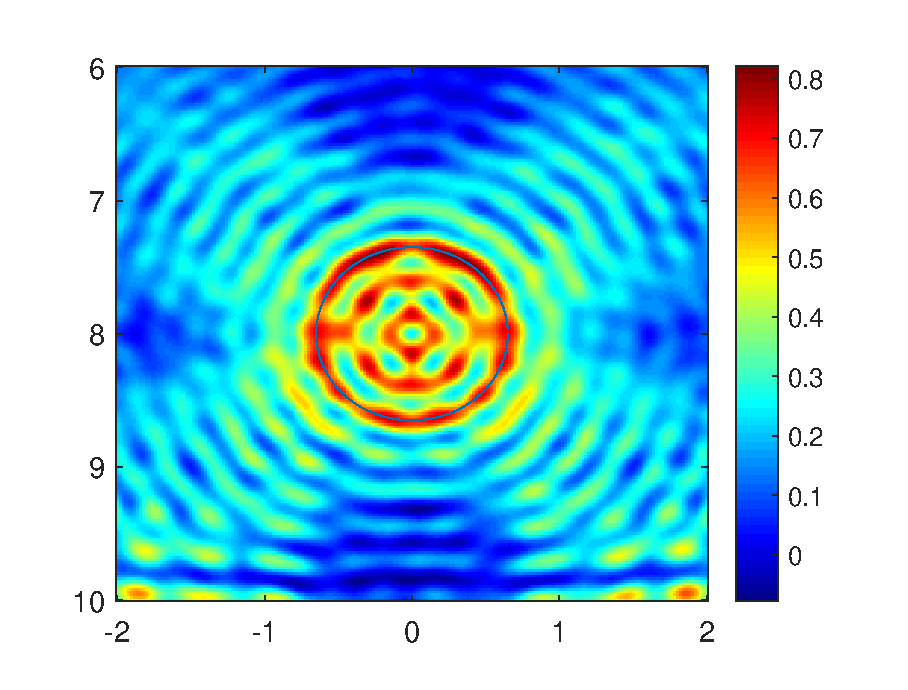
\includegraphics[width=0.23\textwidth]{./waveguide2/example3/circle_transmission_in_2.eps}
  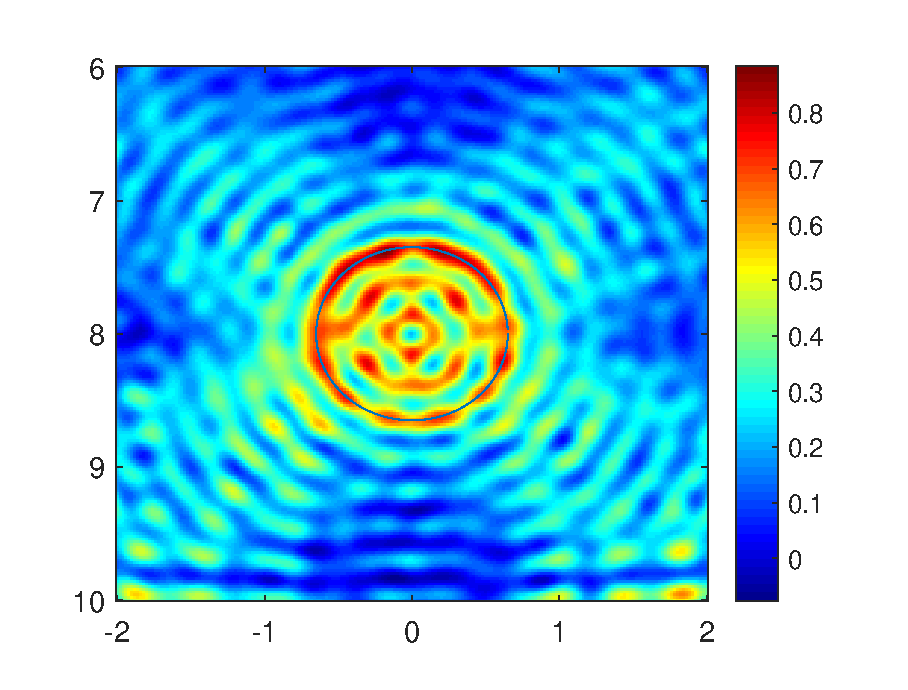
\includegraphics[width=0.23\textwidth]{./waveguide2/example3/circle_transmission_in_4.eps}
  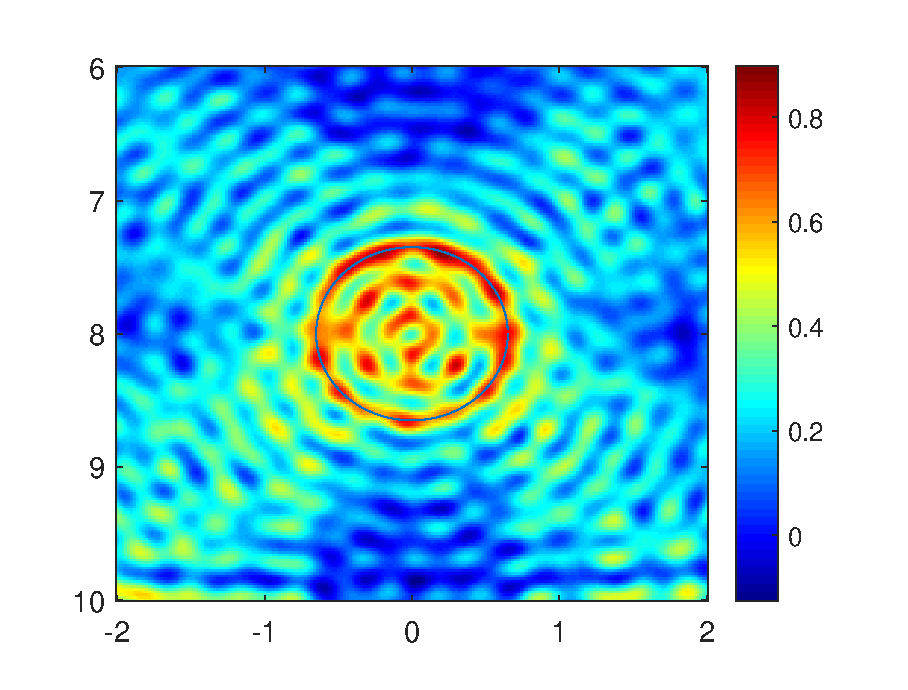
\includegraphics[width=0.23\textwidth]{./waveguide2/example3/circle_transmission_in_6.eps}
  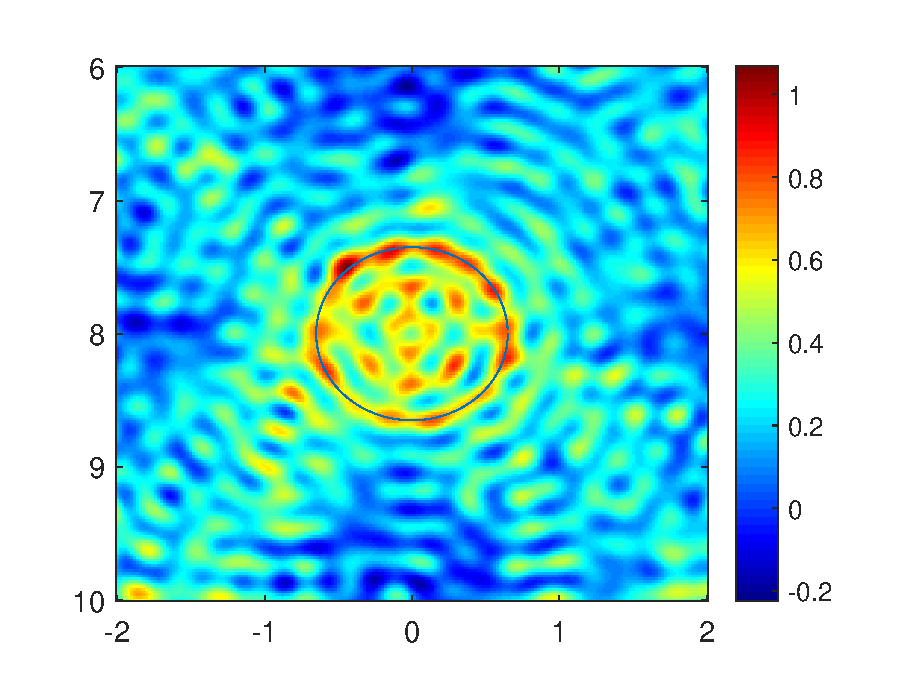
\includegraphics[width=0.23\textwidth]{./waveguide2/example3/circle_transmission_in_8.eps}
  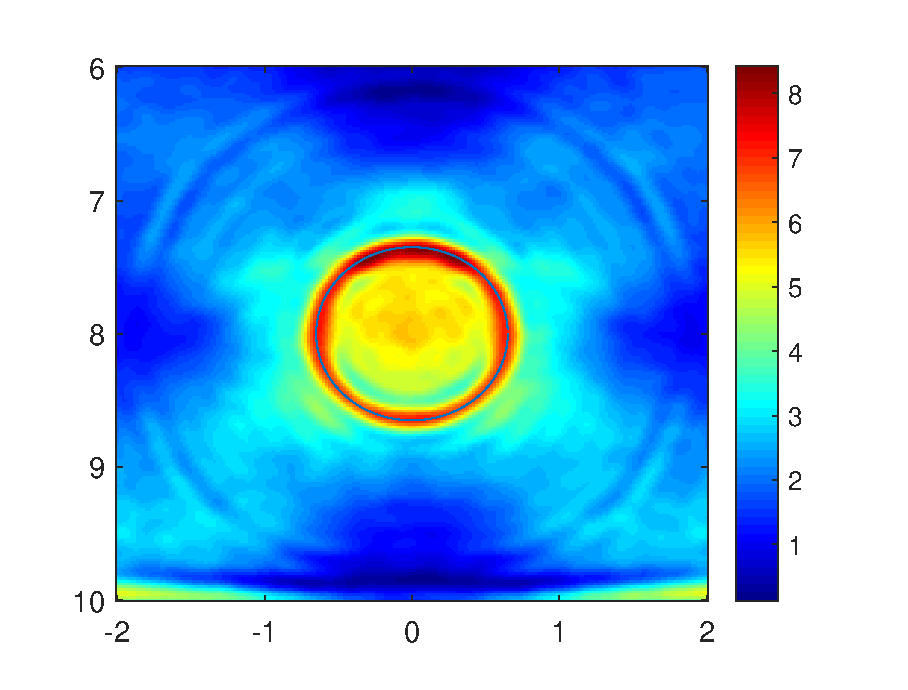
\includegraphics[width=0.23\textwidth]{./waveguide2/example3/circle_transmission_in_2_multi.eps}
  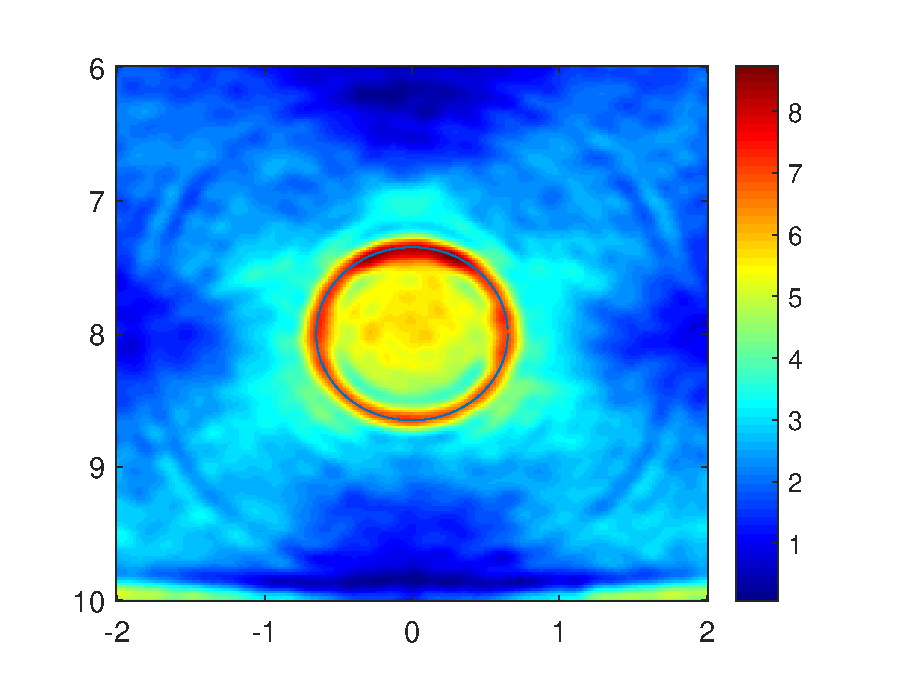
\includegraphics[width=0.23\textwidth]{./waveguide2/example3/circle_transmission_in_4_multi.eps}
  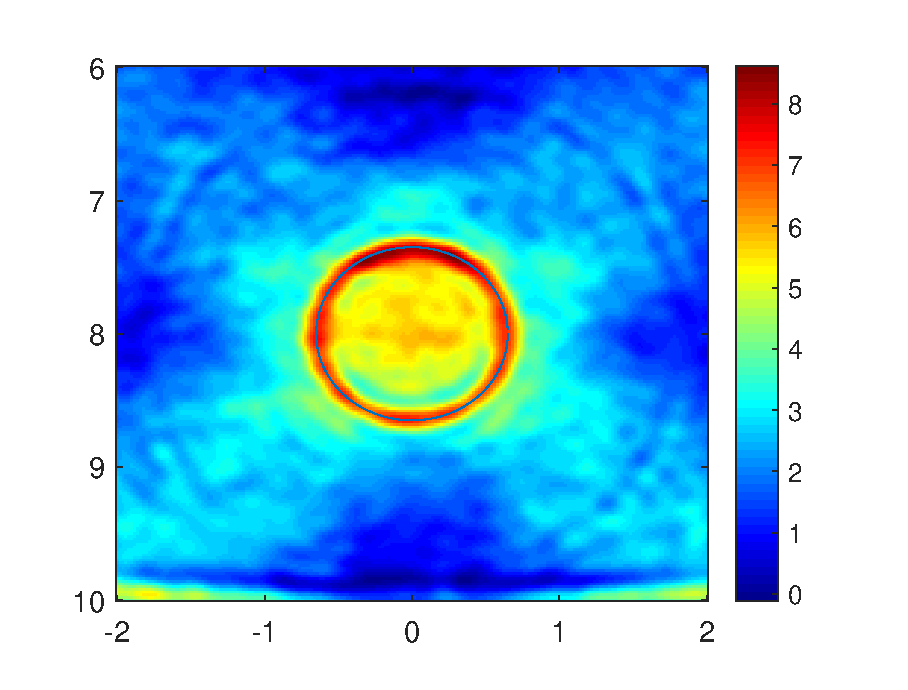
\includegraphics[width=0.23\textwidth]{./waveguide2/example3/circle_transmission_in_6_multi.eps}
  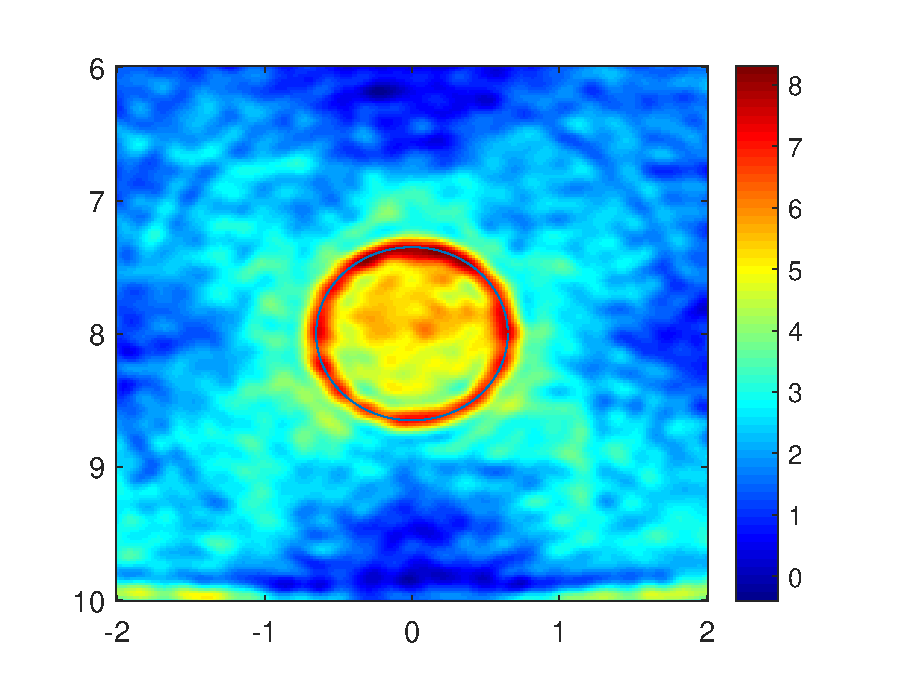
\includegraphics[width=0.23\textwidth]{./waveguide2/example3/circle_transmission_in_8_multi.eps}
   \caption{算例\ref{imp_ex3}:测试算法\ref{alg_imp}对可穿透障碍物成像的抗噪音性能:噪音水平$\mu$从左到右依次按如下数值依次递增:$0.1,0.2,0.4,0.6$。其中第一行为单频测试:$k_1=4\pi,k_2=2\pi,\lambda=2k_1$;第二行为多频测试::$\lambda=2k_1,k_2=\frac{1}{2}k_1,k_1=2\pi+0.4n\pi,n=0,1,\ldots,9$}\label{fig_imp_ex3_2}
\end{figure}
\begin{remark}
	从本小节的数值测试结果可以看出,当障碍物$D$嵌入在Pekeris开波导第一层$L_1$时,阻抗型逆时偏移算法算法\ref{alg_imp}对不同形状不同类型的障碍物都可以做到有效成像。当接收到的数据带有噪音时,算法\ref{alg_imp}具有十分良好的抗噪音能力,并且可以通过对多个频率的成像函数直接相加来改善成像效果,提高抗噪能力。除此之外,数值测试同样表明:
	$D\subset L_1$时,可以考虑选取全空间两层基本解$G_h(x,z)$作为反传播函数,其优点是函数$G_h(x,z)$的表达式\eqref{f_twolayer}相对简单,理论分析和数值计算都相对容易。
\end{remark}
\subsection{$D\subset L_2$.}
在本小节,我们测试当障碍物位于开波导第二层时,算法\ref{alg_imp}的成像效果。我们令$h=10,d=50$,且源点$x_s$ 和接收点$x_r$ 在$\Gamma_0^d$ 上均匀分布,其中$\Gamma_0^d=\{(x_1,x_2)\in\R^2;x_1\in(-d,d),x_2=0\}$。 采样区域为$\Omega=[-2,2]\times[10,14]$,且我们采用$201\times201$ 的均匀采样。探测频率为$k_1=8\pi,k_2=4\pi$。 源点和接收点个数为$N_s=256,N_r=256$。
\begin{example}[不同边界类型]\label{impout_ex1}
在本算例中,我们以圆形障碍物为例,验证算法\ref{alg_imp}对位于Pekeris 开波导第二层具有不同边界类型的障碍物的成像效果。例如声软障碍物,声硬障碍物,折射系数为$n(x)$ 的可穿透障碍物,阻尼系数为$\eta(x)$的阻抗边界障碍物。对于可穿透障碍物成像,我们假设折射系数$n(x)$ 为:
\begin{eqnarray*}
n(x)=\left\{
\begin{array}{lll}
  0.5&,&x\in D\\
  1&,&x\in\R_+^2\backslash\overline D
\end{array}
\right.
\end{eqnarray*}
对于阻抗边界障碍物,我们假设在上半边界$\eta(x)=1$,在下半边界$\eta(x)=2$。除此之外,我们也将使用相同的参数,来测试反传播函数为全空间两层基本解$G_h(x,z)$时所对应成像函数\ref{Id_twolayer}的成像效果。

测试效果如图\ref{fig_impout_ex1}所示:从左到右依次为声软障碍物、声硬障碍物、阻尼系数为$\eta(x)$的阻抗障碍物以及折射系数为$n(x)$的可穿透障碍物,其中第一行为算法\ref{alg_imp}中成像函数\ref{Id_imp}的成像效果,第二行为反传播函数为$G_h(x,z)$的成像函数\ref{Id_twolayer}的成像效果。结果表示:当目标障碍物$D$位于开波导第二层$L_2$时,在没有提前知道障碍物的任何先验信息的情况下,例如是否可穿透,以及不可穿透障碍物的边界条件,两种成像函数都能够对不同类型的障碍物做到有效成像,而且除成像函数值有所差别外,其成像效果都可以与算法\ref{alg_wg}相媲美,达到文献\cite{ch_ha}中一般半空间模型逆时偏移算法的成像效果。
\end{example}
\begin{figure}[h]
  \centering
  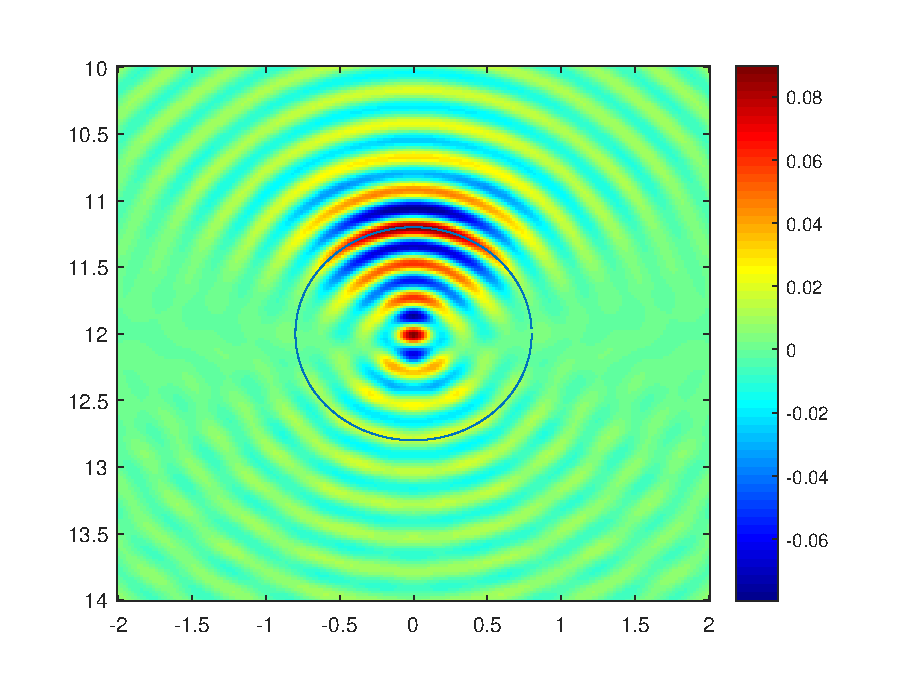
\includegraphics[width=0.23\textwidth]{./waveguide2/out_example1/out_circle_soft_impedance.eps}
  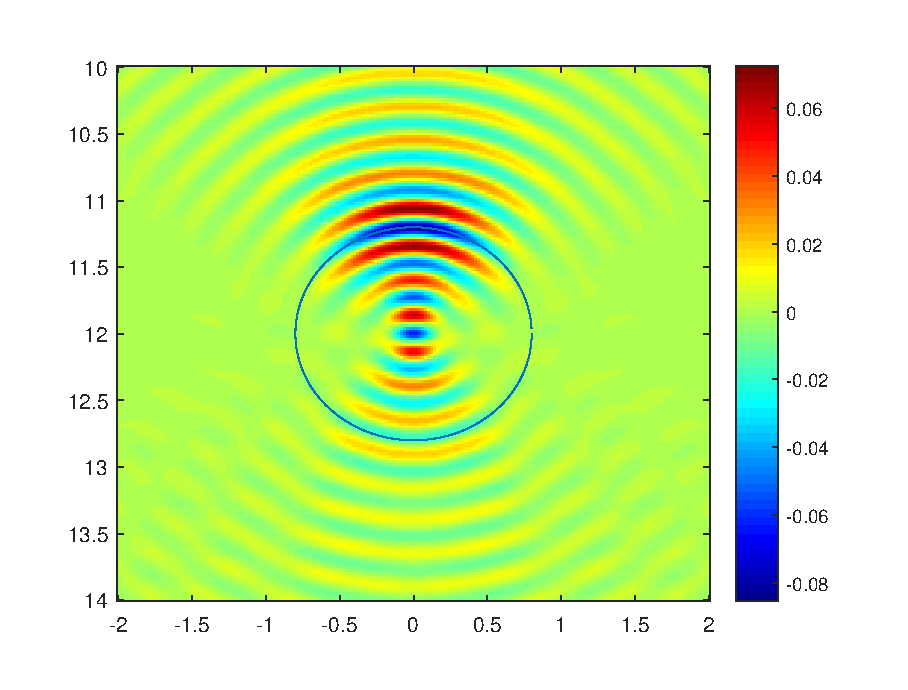
\includegraphics[width=0.23\textwidth]{./waveguide2/out_example1/out_circle_hard_impedance.eps}
  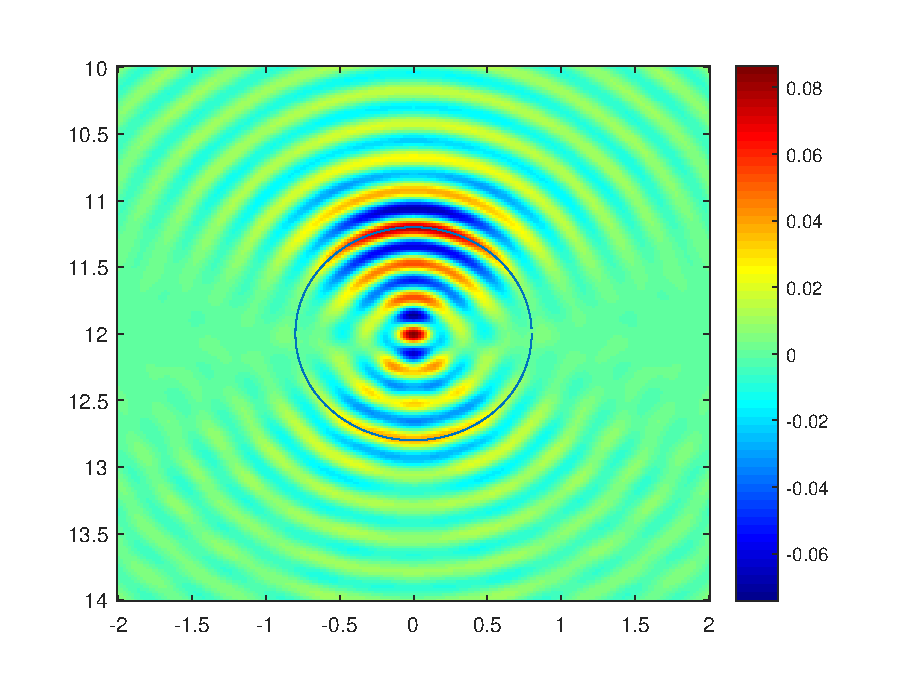
\includegraphics[width=0.23\textwidth]{./waveguide2/out_example1/out_circle_imp_impedance.eps}
  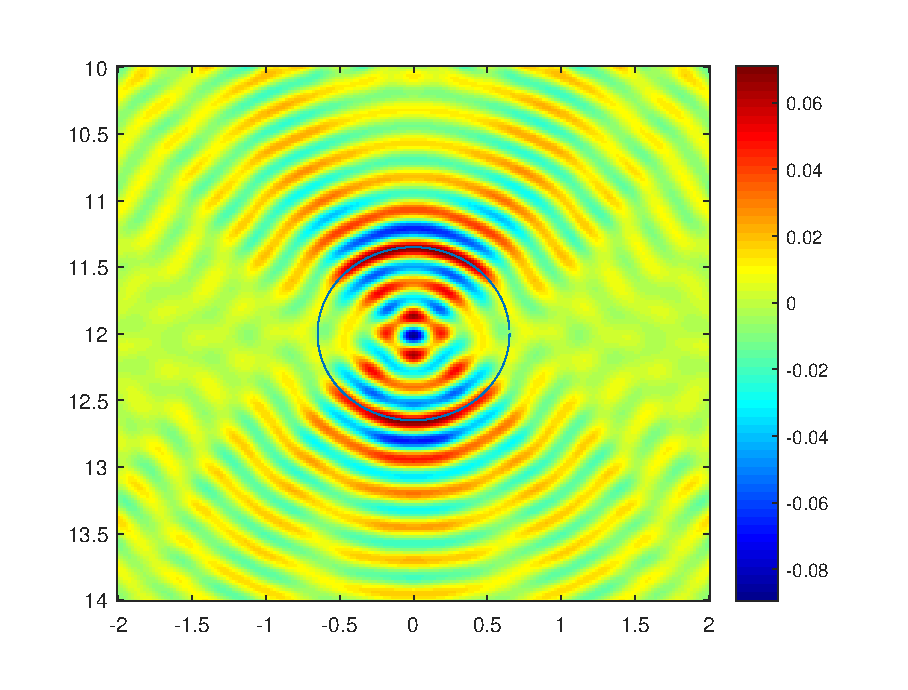
\includegraphics[width=0.23\textwidth]{./waveguide2/out_example1/out_circle_tran_impedance.eps}
  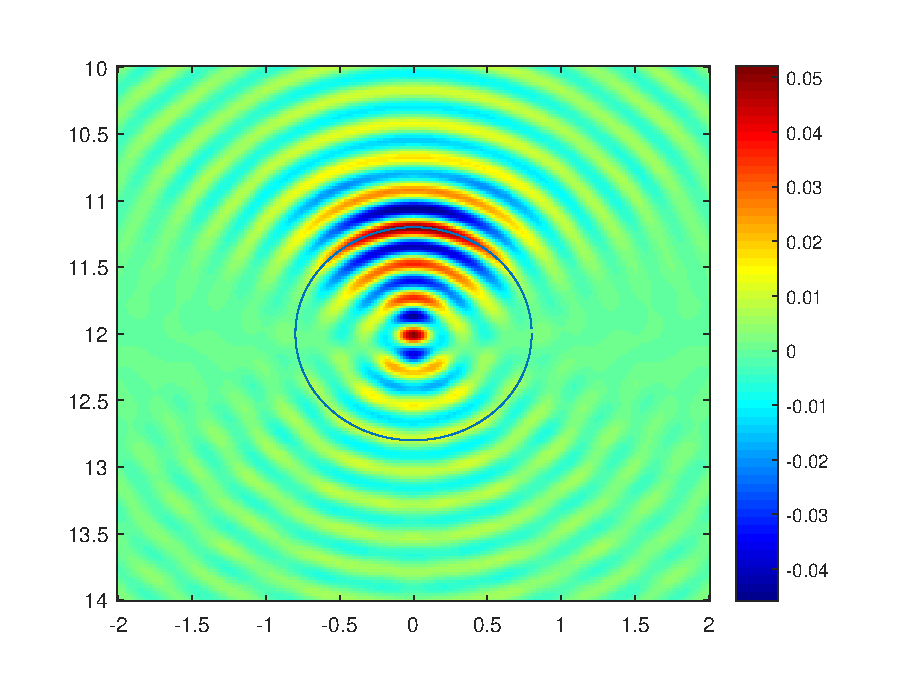
\includegraphics[width=0.23\textwidth]{./waveguide2/out_example1/out_circle_soft_twolayer.eps}
  \includegraphics[width=0.23\textwidth]{./waveguide2/out_example1/out_circle_hard_twolayer.eps}
  \includegraphics[width=0.23\textwidth]{./waveguide2/out_example1/out_circle_imp_twolayer.eps}
  \includegraphics[width=0.23\textwidth]{./waveguide2/out_example1/out_circle_tran_twolayer.eps}
  \caption{算例\ref{impout_ex1}:测试位于$L_2$层的不同类型障碍物:从左到右依次为声软障碍物、声硬障碍物、阻尼系数为$\eta(x)$的阻抗边界障碍物以及折射系数为$n(x)$的可穿透障碍物。其中第一行为算法\ref{alg_imp}的成像效果;第二行是反传播函数为$G_h(x,z)$的成像函数\ref{Id_twolayer}相应的成像效果。}
  \label{fig_impout_ex1}
\end{figure}
\begin{example}[不同形状]\label{impout_ex2}
在本算例中,我们将以声软障碍物和可穿透障碍物为例,来测试算法\ref{alg_imp}对于嵌入在Pekeris 开波导第二层中具有不同形状的障碍物的成像效果。

声软障碍物和可穿透障碍物的测试结果分别如图\ref{fig_imp_ex2_1}和图\ref{fig_imp_ex2_2}所示:从左到右依次为4叶风扇形状,矩形形状,花生形状和椭圆形状,其中每个算例第一行为算法\ref{alg_imp}中成像函数\ref{Id_imp}的测试结果;第二行为取反传播函数为$G_h(x,z)$时所对应成像函数\ref{Id_twolayer}的测试结果。结果表明:当目标障碍物$D$嵌入在开波导第二层$L_2$时,两种成像函数对不同形状的障碍物都能够做到有效成像;而且对于可穿透障碍物,两种成像函数还可以确定其下半边界的位置、大小和形状。
\end{example}
\begin{figure}[h]
  \centering
  \includegraphics[width=0.23\textwidth]{./waveguide2/out_example2/Out_soft_pleaf1_impedance.eps}
  \includegraphics[width=0.23\textwidth]{./waveguide2/out_example2/Out_soft_square1_impedance.eps}
  \includegraphics[width=0.23\textwidth]{./waveguide2/out_example2/Out_soft_peanut_impedance.eps}
  \includegraphics[width=0.23\textwidth]{./waveguide2/out_example2/Out_soft_circle1_impedance.eps}
  \includegraphics[width=0.23\textwidth]{./waveguide2/out_example2/Out_soft_pleaf1_twolayer.eps}
  \includegraphics[width=0.23\textwidth]{./waveguide2/out_example2/Out_soft_square1_twolayer.eps}
  \includegraphics[width=0.23\textwidth]{./waveguide2/out_example2/Out_soft_peanut_twolayer.eps}
  \includegraphics[width=0.23\textwidth]{./waveguide2/out_example2/Out_soft_circle1_twolayer.eps}  
  \caption{算例\ref{impout_ex2}:测试不同形状的声软障碍物:从左到右依次为4-叶风扇、矩形、花生以及椭圆形状,其中第一行为算法\ref{alg_imp}中成像函数\ref{Id_imp}的测试结果;第二行为取反传播函数为$G_h(x,z)$时所对应成像函数\ref{Id_twolayer}的测试结果。}
  \label{fig_imp_ex2_1}
\end{figure}
\begin{figure}[h]
	\centering
	\includegraphics[width=0.23\textwidth]{./waveguide2/out_example2/Out_tran_pleaf1_impedance.eps}
	\includegraphics[width=0.23\textwidth]{./waveguide2/out_example2/Out_tran_square1_impedance.eps}
	\includegraphics[width=0.23\textwidth]{./waveguide2/out_example2/Out_tran_peanut_impedance.eps}
	\includegraphics[width=0.23\textwidth]{./waveguide2/out_example2/Out_tran_circle1_impedance.eps}
	\includegraphics[width=0.23\textwidth]{./waveguide2/out_example2/Out_tran_pleaf1_twolayer.eps}
	\includegraphics[width=0.23\textwidth]{./waveguide2/out_example2/Out_tran_square1_twolayer.eps}
	\includegraphics[width=0.23\textwidth]{./waveguide2/out_example2/Out_tran_peanut_twolayer.eps}
	\includegraphics[width=0.23\textwidth]{./waveguide2/out_example2/Out_tran_circle1_twolayer.eps}  
	\caption{算例\ref{impout_ex2}:测试不同形状的可穿透障碍物:从左到右依次为4-叶风扇、矩形、花生以及椭圆形状,其中第一行为算法\ref{alg_imp}中成像函数\ref{Id_imp}的测试结果;第二行为取反传播函数为$G_h(x,z)$时所对应成像函数\ref{Id_twolayer}的测试结果。}
	\label{fig_imp_ex2_2}
\end{figure}
\begin{example}[抗噪性及多频测试]\label{impout_ex3}
在本算例中,我们测试当在$\Gamma_0^d$上接收到的散射数据$u^s(x_r,x_s)$带有高斯噪音时,对嵌入在Pekeris开波导第二层障碍物,算法\ref{alg_imp}的抗噪性能。假设$u^s_{noise}(x_r,x_s)$ 为如下带有高斯噪音的散射数据:
$$ u^s_{noise}(x_r,x_s)=u^s(x_r,x_s)+v_{noise},$$
其中$v_{noise}$为满足如下分布的高斯噪音:
$$v_{noise}=\mu \max{|u^s|}\epsilon,\ \ \epsilon\sim N(0,1).$$

测试结果如图\ref{fig_impout_ex3}所示:从左到右噪音水平$\mu$按如下数值依次递增:$0.1,0.2,0.4,0.6$。其中第一行为单频测试结果,测试参数为:$k_1=8\pi,k_2=4\pi,\lambda=2k_1$;第二行为多频测试结果,测试参数为:$\lambda=2k_1,k_2=\frac{1}{2}k_1,k_1=2\pi+0.4n\pi,n=0,1,\ldots,9$。结果表示:1. 当目标障碍物$D$嵌入在开波导第二层$L_2$时,算法\ref{alg_imp}具有十分良好的抗噪性能;2. 当采集到的数据为多频信息时,直接将多个频率的成像函数直接相加能够极大地改善算法的成像效果,提高其抗噪能力。
\end{example}
\begin{figure}[h]
  \centering
  \includegraphics[width=0.23\textwidth]{./waveguide2/out_example3/Out_soft_pleaf1_2.eps}
  \includegraphics[width=0.23\textwidth]{./waveguide2/out_example3/Out_soft_pleaf1_4.eps}
  \includegraphics[width=0.23\textwidth]{./waveguide2/out_example3/Out_soft_pleaf1_6.eps}
  \includegraphics[width=0.23\textwidth]{./waveguide2/out_example3/Out_soft_pleaf1_8.eps}
  \includegraphics[width=0.23\textwidth]{./waveguide2/out_example3/Out_soft_pleaf1_2_multi.eps}
  \includegraphics[width=0.23\textwidth]{./waveguide2/out_example3/Out_soft_pleaf1_4_multi.eps}
  \includegraphics[width=0.23\textwidth]{./waveguide2/out_example3/Out_soft_pleaf1_6_multi.eps}
  \includegraphics[width=0.23\textwidth]{./waveguide2/out_example3/Out_soft_pleaf1_8_multi.eps}
  \caption{算例\ref{impout_ex3}:测试算法\ref{alg_imp}的抗噪能力:目标障碍物$D$位于开波导第二层$L_2$内,从左到右噪音水平$\mu$按如下数值依次递增:$0.1,0.2,0.4,0.6$。其中第一行为单频测试:$k_1=8\pi,k_2=4\pi,\lambda=2k_1$;第二行为多频测试$\lambda=2k_1,k_2=\frac{1}{2}k_1,k_1=2\pi+0.4n\pi,n=0,1,\ldots,9$:}\label{fig_impout_ex3}
\end{figure}
\begin{remark}
	从本小节的数值测试可以看出,当目标障碍物$D$嵌入在Pekeris开波导模型第一层$L_2$内时,本章所提算法\ref{alg_imp}中的成像函数\ref{Id_imp}能够对具有不同形状不同类型的障碍物做到有效成像,而且成像效果可以达到文献\cite{ch_ha}中一般半空间逆时偏移算法的水平;其次,算法\ref{alg_imp}具有十分良好的抗噪性能;最后,当所采集到散射数据为多频信息时,直接将多个频率的成像函数\ref{Id_imp}相加,能够极大地改善成像效果,并提升算法的抗噪性能。
	
	除此之外,通过数值测试,我们还发现,如果问题模型仅仅为半空间两层介质的Pekeris开波导模型,那么选取全空间两层基本解$G_h(x,z)$来计算反传播场和互相关关系,可以达到相同的成像效果,其优点在于函数$G_h(x,z)$的表达式\eqref{f_twolayer}相对简单,理论分析和数值测试相对容易。
\end{remark}
%\section{算法分析与解释}
%\section{本章小结}


